% =========================================================================================
%                                  KHAI BÁO CLASS VÀ GÓI LỆNH
% =========================================================================================
\documentclass[12pt, a4paper]{report}

% --- 1. Font chữ & Ngôn ngữ ---
\usepackage{mathptmx}           % Font Times New Roman
\usepackage[utf8]{vietnam}      % Hỗ trợ tiếng Việt
% \usepackage{fontsize}           % Gói lệnh để chỉnh cỡ chữ tùy ý
% \changefontsize[16pt]{13pt}       % Thiết lập: Cỡ chữ 13pt, giãn dòng 16pt (khoảng 1.2 lần)
% --- 2. Toán học & Ký hiệu ---
\usepackage{amsmath}            % Các phép toán
\usepackage{amssymb, latexsym}  % Ký hiệu toán học
\usepackage{array, hhline}      % Bảng biểu nâng cao

% --- 3. Đồ họa & Hình ảnh ---
\usepackage{graphicx}           % Chèn hình ảnh
\usepackage{tikz}               % Vẽ hình vector mạnh mẽ
\usetikzlibrary{arrows.meta,shapes,positioning,calc,fit} % Thư viện mở rộng của TikZ
\usepackage[framemethod=tikz]{mdframed} % Khung đoạn văn

% --- 4. Định dạng trang & Bố cục ---
\usepackage[a4paper, top=2cm, bottom=2cm, left=3cm, right=2cm]{geometry} % Căn lề
\usepackage{parskip}            % Tạo khoảng cách giữa các đoạn văn
\usepackage{lastpage}           % Đếm tổng số trang
\usepackage{fancyhdr}           % Tạo Header/Footer tùy chỉnh
\usepackage{titlesec}           % Chỉnh sửa tiêu đề Chapter/Section
\usepackage{caption, subcaption}% Chú thích hình ảnh
\usepackage{tabularx}           % Bảng co giãn
\usepackage{pgfgantt} % biểu đồ Gantt
% --- 5. Tiện ích & Code ---
\usepackage{listings}           % Chèn code (C++, Python...)
\usepackage{attachfile}         % Đính kèm file
\usepackage{hyperref}           % Tạo bookmark và link

%---6 Tài liệu tham khảo -------
\usepackage[
    backend=biber, 
    style=ieee,     % ieee hoặc numeric sẽ cho ra dạng [1], [2]
    sorting=none     % Sắp xếp theo Name - Title - Year
]{biblatex}
\addbibresource{tailieu.bib}
% =========================================================================================
%                                  CẤU HÌNH GIAO DIỆN (SETTINGS)
% =========================================================================================

% --- 1. Cấu hình Code Listing (Màu sắc & Style) ---
\definecolor{codegreen}{rgb}{0,0.6,0}
\definecolor{codegray}{rgb}{0.5,0.5,0.5}
\definecolor{codepurple}{rgb}{0.58,0,0.82}
\definecolor{backcolour}{rgb}{0.95,0.95,0.92}
\definecolor{light-gray}{gray}{0.95}

\lstdefinestyle{mystyle}{
    backgroundcolor=\color{backcolour},   
    commentstyle=\color{codegreen},
    keywordstyle=\color{magenta},
    numberstyle=\tiny\color{codegray},
    stringstyle=\color{codepurple},
    basicstyle=\ttfamily\footnotesize,
    breakatwhitespace=false,         
    breaklines=true,                 
    captionpos=b,                    
    keepspaces=true,                 
    numbers=left,                    
    numbersep=5pt,                  
    showspaces=false,                
    showstringspaces=false,
    showtabs=false,                  
    tabsize=2
}
\lstset{style=mystyle}
\newcommand{\code}[1]{\colorbox{light-gray}{\texttt{#1}}}

% --- 2. Cấu hình Chapter (Số to, kẻ ngang) ---
\titleformat{\chapter}[display]
  {\normalfont} 
  {%
    \bfseries\LARGE\MakeUppercase{\chaptertitlename} 
    \ \fontsize{30}{30}\selectfont\thechapter 
  }
  {0.5ex} 
  {%
    \titlerule 
    \vspace{1ex}
    \filleft 
    \bfseries\Large\MakeUppercase 
  }
  [%
    \vspace{1ex} 
    \titlerule 
  ]
\titlespacing*{\chapter}{0pt}{0pt}{30pt}

% --- 3. Cấu hình Header & Footer ---
\setlength{\headheight}{20pt} 
\pagestyle{fancy}
\fancyhf{} % Xóa sạch cấu hình cũ

% --- A. Định nghĩa nội dung lưu vào bộ nhớ ---
% Chúng ta chỉ cần lưu Section vào bộ nhớ \leftmark để hiện ở góc trái
\renewcommand{\chaptermark}[1]{\markboth{}{}} 
\renewcommand{\sectionmark}[1]{\markboth{\thesection.\ #1}{}} 

% --- B. Hiển thị Header (Giống nhau cho TẤT CẢ các trang) ---
% [L] = Left (Trái), [R] = Right (Phải) -> Áp dụng cho cả chẵn và lẻ
\fancyhead[L]{\itshape\nouppercase{\leftmark}} % Hiện tên Section
\fancyhead[R]{\textbf{\thepage}}               % Hiện số trang

% --- C. Đường kẻ ---
\renewcommand{\headrulewidth}{0.5pt}

% --- 4. Cấu hình Mục lục (Độ sâu) ---
\setcounter{secnumdepth}{4} % Đánh số tới cấp 4 (subsubsubsection)
\setcounter{tocdepth}{2}    % Hiện mục lục tới cấp 2

% =========================================================================================
%                                  NỘI DUNG CHÍNH (DOCUMENT)
% =========================================================================================
\begin{document}
% --- PHẦN 1: TRANG BÌA (FRONT MATTER) ---
\thispagestyle{empty}
\begin{titlepage}
    % Chỉnh lề riêng cho trang bìa
    \newgeometry{top=2cm, bottom=2cm, left=1.5cm, right=1.5cm}
    
    % Vẽ khung viền
    \begin{tikzpicture}[remember picture, overlay]
      \draw[line width=1pt] 
        ($(current page.north west) + (1cm,-1cm)$) rectangle 
        ($(current page.south east) + (-1cm,1cm)$);
      \draw[line width=0.5pt]
        ($(current page.north west) + (1.2cm,-1.2cm)$) rectangle 
        ($(current page.south east) + (-1.2cm,1.2cm)$);
    \end{tikzpicture}
    
    % Nội dung chữ
    \centering
    \textbf{\Large ĐẠI HỌC QUỐC GIA THÀNH PHỐ HỒ CHÍ MINH} \\
    \textbf{\Large TRƯỜNG ĐẠI HỌC BÁCH KHOA} \\
    \textbf{\Large KHOA KHOA HỌC \& KỸ THUẬT MÁY TÍNH} \\
    \vspace{1cm}
    
\includegraphics[width=5cm]{images/hcmut.png} \\
    \vspace{0.5cm}
    
    \huge \text{\textbf{Báo cáo Đồ án}}\\
    \rule{0.8 \linewidth}{0.5mm} \\
    \vspace{0.5cm}
    
    {\LARGE\text{Phát triển Platform EDGE-AI}\\
    \LARGE\text{trên nền tảng FPGA sử dụng RISC-V}}
    \vspace{0.5cm}
    \rule{0.8 \linewidth}{0.5mm}
    \vspace{0.5cm}
    \text{\Large\textbf{Ngành: Kỹ thuật máy tính}} \\
    \vspace{1cm}
    
    % Thông tin GVHD & SV
\begin{flushright}
        \begin{minipage}{0.55\textwidth} % Tạo một khối rộng 55% bề ngang trang
            \Large % Thiết lập cỡ chữ cho toàn bộ khối
            \textbf{Hội đồng báo cáo:} Hội đồng 5L \\
            \rule{0.8 \linewidth}{0.5mm}
            \textbf{GVHD:} Phạm Quốc Cường\\
            \textbf{Sinh viên:} Nguyễn Trung Tân - 2213063\\
            \textbf{Sinh viên:} Trần Minh Tâm - 2213039
        \end{minipage}
    \end{flushright}
                    
    \vspace{2cm}
    \text{\Large{Tp. Hồ Chí Minh 12/2025}}
\end{titlepage}
% Kết thúc trang bìa, trả lại lề chuẩn
\restoregeometry 

% --- PHẦN 2: CÁC TRANG ĐẦU (PREAMBLE PAGES) ---
\newpage
\setlength{\spaceskip}{0.4em plus 0.2em minus 0.2em}
\fontsize{13pt}{18pt}\selectfont
\pagenumbering{gobble} % Tắt đánh số trang
% \begin{center}
    \textbf{\Large Giáo viên hướng dẫn nhận xét}
\end{center}
\makebox[\textwidth]{\dotfill}\\[6pt]
\makebox[\textwidth]{\dotfill}\\[6pt]
\makebox[\textwidth]{\dotfill}\\[6pt]
\makebox[\textwidth]{\dotfill}\\[6pt]
\makebox[\textwidth]{\dotfill}\\[6pt]
\makebox[\textwidth]{\dotfill}\\[6pt]
\makebox[\textwidth]{\dotfill}\\[6pt]
\makebox[\textwidth]{\dotfill}\\[6pt]
\makebox[\textwidth]{\dotfill}\\[6pt]
\makebox[\textwidth]{\dotfill}\\[6pt]

\vspace{8cm}
\begin{flushright}
    \textbf{\Large Giáo viên}
\end{flushright}

\begin{center}
   \textbf{\LARGE Lời cam đoan} 
\end{center}
\vspace{2cm}
Nhóm khẳng định rằng mọi nội dung và thông tin trong báo cáo này đều hoàn toàn trung thực và được thực hiện một cách độc lập. Chúng tôi đảm bảo không  có hành vi gian lận hay sử dụng thông tin từ các nguồn khác mà không được ghi chú rõ ràng trong tài liệu. Mọi tham khảo đến công trình của người khác đều được trích dẫn đầy đủ, và các nguồn thông tin đều được trình bày chính xác theo quy định của hệ thống tham chiếu đã được áp dụng.
Chúng tôi nhận thức rõ ràng việc vi phạm các nguyên tắc về trung thực và minh bạch có thể gây ra những hậu quả nghiêm trọng. Vì vậy, chúng tôi cam kết tuân thủ chặt chẽ mọi quy tắc và chuẩn mực đạo đức liên quan đến việc nghiên cứu và lập báo cáo
\begin{center}
    \textbf{\LARGE Lời cảm ơn}
\end{center}
\vspace{2cm}
Việc hoàn thành đồ án này không chỉ là kết quả của sự nỗ lực từ phía nhóm thực hiện, mà còn là sự kết tinh từ sự chỉ dẫn tận tình và động viên to lớn của quý thầy cô, gia đình và bạn bè.

Lời tri ân sâu sắc nhất, chúng tôi xin được gửi tới Thầy Phạm Quốc Cường. Thầy không chỉ là người hướng dẫn khoa học, định hướng cho chúng tôi những lối đi đúng đắn trong mê cung kiến thức, mà còn là người truyền lửa, giúp chúng tôi kiên trì vượt qua những rào cản kỹ thuật hóc búa trong suốt quá trình thực hiện đề tài. Những kinh nghiệm quý báu mà Thầy chia sẻ thực sự là hành trang vô giá đối với chúng tôi.

Chúng tôi cũng xin bày tỏ lòng biết ơn chân thành đến Quý Thầy Cô thuộc Khoa Khoa học và Kỹ thuật Máy tính, Trường Đại học Bách Khoa - ĐHQG TP.HCM. Môi trường học thuật nghiêm túc và nền tảng kiến thức vững chắc mà các Thầy Cô đã dày công vun đắp chính là bệ phóng để chúng tôi có thể tự tin giải quyết các vấn đề trong đồ án này cũng như trong sự nghiệp sau này.

Cuối cùng, xin gửi lời cảm ơn đến gia đình – hậu phương vững chắc nhất, và những người bạn đã luôn sát cánh, chia sẻ khó khăn. Sự ủng hộ của mọi người chính là nguồn động lực tinh thần to lớn giúp chúng tôi đi đến cuối hành trình này.

Xin chân thành cảm ơn!
\vspace{1cm}
\begin{flushright}
    \textbf{\LARGE Tóm tắt}
\end{flushright}
\vspace{1cm}
Trong kỷ nguyên số hóa, Internet vạn vật (IoT) đã chuyển mình từ một khái niệm công nghệ trở thành hạ tầng thiết yếu của đời sống hiện đại. Từ các thiết bị dân dụng như Smart TV đến các mạng lưới cảm biến công nghiệp phức tạp, IoT đang tạo ra một lượng dữ liệu khổng lồ. Xu hướng tất yếu hiện nay là tích hợp Trí tuệ nhân tạo (AI) vào các thiết bị này để tạo nên AIoT (Artificial Intelligence of Things), giúp thiết bị không chỉ "kết nối" mà còn có khả năng "tư duy".

Tuy nhiên, việc triển khai AI trên các thiết bị IoT truyền thống đang vấp phải "nút thắt cổ chai" về kiến trúc. Mô hình phổ biến hiện nay dựa vào việc đẩy dữ liệu lên máy chủ đám mây (Cloud Server) để xử lý tập trung. Mô hình này bộc lộ nhiều điểm yếu chí mạng: rủi ro gián đoạn dịch vụ khi mất kết nối mạng, độ trễ cao không phù hợp cho các ứng dụng thời gian thực, và gánh nặng băng thông lớn.

Về mặt phần cứng, các vi xử lý (CPU) thương mại từ các hãng lớn, dù mạnh mẽ, thường gặp vấn đề về tiêu thụ năng lượng khi phải gồng gánh các tác vụ AI liên tục. Hơn nữa, tính chất đóng kín của các dòng chip này khiến các nhà phát triển gặp khó khăn trong việc tùy biến sâu để tối ưu hóa hiệu năng cho các thuật toán AI cụ thể, đồng thời rào cản chi phí bản quyền cũng là một trở ngại lớn cho đổi mới sáng tạo.

Sự xuất hiện của RISC-V đã mang đến một luồng gió mới cho ngành công nghiệp bán dẫn. Là một kiến trúc tập lệnh mở (Open ISA), RISC-V phá bỏ thế độc quyền của các kiến trúc đóng, trao quyền cho các tổ chức nhỏ, các nhóm nghiên cứu và cá nhân khả năng tự thiết kế các lõi CPU chuẩn hóa. Ưu điểm vượt trội của RISC-V nằm ở tính mô-đun hóa và khả năng mở rộng. Các kỹ sư có thể tự do thêm các tập lệnh tùy chỉnh hoặc sửa đổi vi kiến trúc để phục vụ cho các tác vụ chuyên biệt mà không vướng phải rào cản pháp lý hay chi phí bản quyền đắt đỏ. Đây chính là chìa khóa để giải quyết bài toán hiệu năng/năng lượng cho các thiết bị IoT thế hệ mới.

Dựa trên những phân tích trên, dự án của nhóm tập trung phát triển một nền tảng Edge-AI (AI tại biên) chuyên dụng, lấy kiến trúc RISC-V làm nòng cốt. Mục tiêu của nhóm không chỉ dừng lại ở việc sử dụng một lõi CPU đa năng. Thay vào đó, nhóm tận dụng khả năng tùy biến của RISC-V để thiết kế một hệ thống tích hợp sâu, bao gồm một lõi xử lý trung tâm được tối ưu hóa kết hợp với một bộ tăng tốc AI tùy chỉnh


\newpage
\tableofcontents % Mục lục
\listoffigures   % Danh sách hình
\listoftables
% --- PHẦN 3: NỘI DUNG BÁO CÁO (MAIN CONTENT) ---
\newpage
\pagenumbering{arabic} % Bắt đầu đánh số 1, 2, 3...
\setcounter{page}{1}

\include{intro}
\chapter{Cơ sở lý thuyết}

\section{Kiến trúc tập lệnh RISC-V}

\subsection{Lịch sử hình thành}

RISC-V là một kiến trúc tập lệnh (Instruction Set Architecture - ISA) 
dựa trên nguyên lý RISC (Reduced Instruction Set Computer), 
được đưa ra vào năm 2010 tại Phòng thí nghiệm Tính toán song song 
của Đại học California, Berkeley. Dự án được dẫn dắt bởi 
Giáo sư Krste Asanović cùng với sự tham gia của hai sinh viên cao học 
là Yunsup Lee và Andrew Waterman, dưới sự cố vấn của David Patterson – cha đẻ 
của kiến trúc RISC nguyên thủy.

Khác với các thế hệ RISC trước đó (như RISC-I, II, III, IV) vốn được 
thiết kế chủ yếu cho mục đích nghiên cứu học thuật, RISC-V ngay từ đầu đã 
được định hướng để trở thành một chuẩn ISA tiêu chuẩn cho cả nghiên cứu lẫn 
thương mại hóa. Mục tiêu của nhóm thiết kế là tạo ra một tập lệnh "sạch", 
không chịu gánh nặng của các vấn đề tương thích ngược từ các kiến trúc cũ kỹ 
tồn tại hàng thập kỷ, đồng thời hoàn toàn mở và miễn phí.

Năm 2015, RISC-V Foundation (nay là RISC-V International) được thành 
lập để quản lý chuẩn hóa và thúc đẩy hệ sinh thái phần cứng/phần mềm. 
Sự ra đời của RISC-V đã phá vỡ thế độc quyền lâu năm của các kiến trúc 
đóng như x86 (Intel) và ARM, mở ra kỷ nguyên "phần cứng mã nguồn mở" 
(Open Source Hardware).

\subsection{Các đặc điểm nổi bật}
So với các kiến trúc thương mại phổ biến, RISC-V sở hữu các đặc điểm kỹ 
thuật và pháp lý vượt trội:
\begin{itemize}
    \item \textbf{Tính mở và Miễn phí (Open \& Free):} RISC-V được phát hành dưới giấy phép BSD. Bất kỳ cá nhân hay tổ chức nào cũng có thể thiết kế, sản xuất và thương mại hóa chip RISC-V mà không phải trả phí bản quyền (Royalty-free). Điều này giúp giảm đáng kể chi phí khởi tạo cho các dự án khởi nghiệp và nghiên cứu.
    \item \textbf{Tính Mô đun:} Thay vì bắt buộc phải hiện thực toàn bộ tập lệnh khổng lồ, RISC-V có lõi là tập lệnh số nguyên cơ sở (Base Integer ISA) rất nhỏ gọn. Các tính năng nâng cao như số thực, nhân chia, hay nén lệnh (Compressed) được coi là các phần mở rộng tùy chọn. Điều này cho phép tối ưu hóa diện tích vi mạch cho các ứng dụng nhúng nhỏ gọn.
    \item \textbf{Khả năng mở rộng (Extensibility):} RISC-V dành riêng một phần không gian mã hóa lệnh (Opcode space) cho người dùng tự định nghĩa. Điều này đặc biệt quan trọng đối với các ứng dụng Edge AI, nơi các kỹ sư có thể thêm các lệnh tính toán ma trận hoặc tích chập chuyên biệt để tăng tốc phần cứng mà không vi phạm chuẩn ISA.
    \item \textbf{Kiến trúc Load/Store thuần túy:} Tương tự các kiến trúc RISC khác, RISC-V tách biệt hoàn toàn việc truy cập bộ nhớ và xử lý dữ liệu, giúp đơn giản hóa thiết kế phần cứng của Pipeline.
\end{itemize}

\subsection{Cấu trúc tập lệnh cơ sở và các phần mở rộng}

\subsubsection{Tập lệnh số nguyên cơ sở (Base Integer ISA)}
Nền tảng của RISC-V là tập lệnh số nguyên cơ sở, được ký hiệu là \textbf{RV32I} (cho bản 32-bit), RV64I (64-bit) hoặc RV128I (128-bit). Trong phạm vi đồ án này, nhóm tập trung vào \textbf{RV32I}, bao gồm 47 lệnh cơ bản.

\textbf{Hệ thống thanh ghi (Register File):}
RV32I cung cấp 32 thanh ghi đa năng (General Purpose Registers - GPR), mỗi thanh ghi rộng 32-bit, được đánh số từ $x0$ đến $x31$. Ngoài ra còn có một thanh ghi đếm chương trình (Program Counter - PC).

Theo quy ước gọi hàm (Calling Convention) của RISC-V ABI, các thanh ghi này có vai trò cụ thể như mô tả trong Bảng \ref{tab:riscv_registers}:

\begin{table}[h]
\centering
\begin{tabular}{|l|l|l|l|}
\hline
\textbf{Tên} & \textbf{ABI Name} & \textbf{Mô tả} & \textbf{Lưu bởi} \\ \hline
x0 & zero & Luôn có giá trị bằng 0 (Hardwired Zero) & - \\ \hline
x1 & ra & Địa chỉ trả về (Return Address) & Caller \\ \hline
x2 & sp & Con trỏ ngăn xếp (Stack Pointer) & Callee \\ \hline
x3 & gp & Con trỏ toàn cục (Global Pointer) & - \\ \hline
x4 & tp & Con trỏ luồng (Thread Pointer) & - \\ \hline
x5-x7 & t0-t2 & Thanh ghi tạm thời (Temporaries) & Caller \\ \hline
x8 & s0/fp & Thanh ghi lưu trữ/Con trỏ khung (Frame Ptr) & Callee \\ \hline
x9 & s1 & Thanh ghi lưu trữ (Saved Register) & Callee \\ \hline
x10-x11 & a0-a1 & Tham số hàm / Giá trị trả về & Caller \\ \hline
x12-x17 & a2-a7 & Tham số hàm (Function Arguments) & Caller \\ \hline
x18-x27 & s2-s11 & Thanh ghi lưu trữ (Saved Registers) & Callee \\ \hline
x28-x31 & t3-t6 & Thanh ghi tạm thời (Temporaries) & Caller \\ \hline
\end{tabular}
\caption{Quy ước sử dụng thanh ghi trong RISC-V (ABI)}
\label{tab:riscv_registers}
\end{table}

\subsubsection{Định dạng lệnh (Instruction Formats)}
Để đơn giản hóa bộ giải mã, các lệnh trong RV32I có độ dài cố định 32-bit và được căn chỉnh bộ nhớ (aligned) theo địa chỉ chia hết cho 4. RISC-V định nghĩa 6 định dạng lệnh cơ bản:

\begin{itemize}
    \item \textbf{R-type (Register):} Dùng cho các phép toán giữa các thanh ghi (VD: cộng, trừ, logic). Cấu trúc gồm: opcode, rd (đích), funct3, rs1 (nguồn 1), rs2 (nguồn 2), funct7.
    \item \textbf{I-type (Immediate):} Dùng cho các phép toán với hằng số ngắn hoặc lệnh Load. Gồm: opcode, rd, funct3, rs1, imm[11:0].
    \item \textbf{S-type (Store):} Dùng cho lệnh lưu dữ liệu ra bộ nhớ (Store). Hằng số immediate được chia làm 2 phần để giữ vị trí các thanh ghi nguồn cố định.
    \item \textbf{B-type (Branch):} Dùng cho các lệnh rẽ nhánh có điều kiện. Tương tự S-type nhưng immediate được mã hóa khác để mở rộng phạm vi nhảy.
    \item \textbf{U-type (Upper Immediate):} Dùng cho lệnh thao tác với 20-bit cao của thanh ghi (VD: LUI, AUIPC).
    \item \textbf{J-type (Jump):} Dùng cho lệnh nhảy không điều kiện (JAL).
\end{itemize}


\subsubsection{Các chế độ đặc quyền}
RISC-V định nghĩa ba chế độ đặc quyền để bảo vệ hệ thống:
\begin{enumerate}
    \item \textbf{Machine Mode (M-Mode):} Chế độ có quyền cao nhất, truy cập toàn bộ tài nguyên phần cứng. Các vi điều khiển đơn giản (bare-metal) chỉ cần chạy ở chế độ này.
    \item \textbf{Supervisor Mode (S-Mode):} Dùng cho hệ điều hành (như Linux, FreeRTOS) để quản lý bộ nhớ ảo và bảo vệ tài nguyên.
    \item \textbf{User Mode (U-Mode):} Chế độ có quyền thấp nhất, dành cho các ứng dụng người dùng.
\end{enumerate}
Trong đồ án này, lõi RISC-V chủ yếu sẽ hoạt động ở M-Mode để tương tác trực tiếp với phần cứng FPGA và bộ tăng tốc.


\subsection{So sánh kiến trúc RISC và CISC}

Để làm rõ ưu thế của việc lựa chọn RISC-V cho đề tài, cần đặt nó vào hệ quy chiếu so sánh với kiến trúc CISC (Complex Instruction Set Computer) – triết lý thiết kế đối lập vốn thống trị thị trường máy tính cá nhân (PC) nhiều thập kỷ qua.

\subsubsection{Triết lý thiết kế}
Sự khác biệt căn bản giữa RISC và CISC nằm ở cách phân chia khối lượng công việc giữa phần cứng (Hardware) và phần mềm (Software/Compiler):

\begin{itemize}
    \item \textbf{CISC:} Tập trung vào việc giảm "khoảng cách ngữ nghĩa" (semantic gap) giữa ngôn ngữ bậc cao và mã máy. CISC cung cấp các lệnh phức tạp, đa năng (ví dụ: một lệnh duy nhất có thể thực hiện nạp dữ liệu, cộng và lưu kết quả). Điều này giúp giảm kích thước mã chương trình (Code size) nhưng làm tăng độ phức tạp của phần cứng giải mã lệnh.
    \item \textbf{RISC:} Chuyển gánh nặng tối ưu hóa sang trình biên dịch (Compiler). Tập lệnh chỉ bao gồm các chỉ thị đơn giản, thực thi nhanh. Các tác vụ phức tạp được thực hiện bằng cách kết hợp nhiều lệnh đơn giản. Điều này giúp phần cứng đơn giản hơn, tiết kiệm diện tích silicon để dành cho bộ nhớ đệm (Cache) hoặc các lõi xử lý song song.
\end{itemize}



\subsubsection{So sánh RISC và CISC}
Bảng \ref{tab:risc_vs_cisc} tóm tắt các đặc điểm kỹ thuật đối lập giữa hai kiến trúc \cite{risc-v}:

\begin{table}[h]
\centering
\begin{tabular}{|p{4cm}|p{5.5cm}|p{5.5cm}|}
\hline
\textbf{Tiêu chí} & \textbf{RISC (RISC-V, ARM)} & \textbf{CISC (x86)} \\ \hline
\textbf{Độ phức tạp lệnh} & Đơn giản, thực hiện tác vụ nhỏ. & Phức tạp, một lệnh làm nhiều việc (truy cập bộ nhớ, tính toán). \\ \hline
\textbf{Thời gian thực thi} & Hướng tới 1 chu kỳ máy/lệnh (CPI $\approx$ 1). & Đa chu kỳ (Multi-cycle), số chu kỳ thay đổi tùy lệnh. \\ \hline
\textbf{Định dạng lệnh} & Cố định (thường là 32-bit), giải mã nhanh. & Thay đổi (Variable length), giải mã phức tạp. \\ \hline
\textbf{Truy cập bộ nhớ} & Chỉ qua lệnh Load/Store. & Các lệnh tính toán có thể thao tác trực tiếp với bộ nhớ. \\ \hline
\textbf{Số lượng thanh ghi} & Nhiều (32 hoặc hơn) để giảm truy cập RAM. & Ít thanh ghi chuyên dụng hơn. \\ \hline
\textbf{Pipiline} & Dễ dàng hiện thực và đạt hiệu quả cao. & Khó hiện thực do độ dài lệnh không đồng nhất. \\ \hline
\textbf{Kích thước chương trình} & Lớn hơn (cần nhiều lệnh để làm một việc). & Nhỏ gọn hơn (mật độ mã cao). \\ \hline
\end{tabular}
\caption{So sánh đặc điểm kỹ thuật giữa RISC và CISC}
\label{tab:risc_vs_cisc}
\end{table}

\subsection{Các phần mở rộng tiêu chuẩn (Standard Extensions)}
Để tăng cường khả năng xử lý, RISC-V cung cấp các phần mở rộng được chuẩn hóa. Một vi xử lý hỗ trợ đầy đủ các mở rộng cơ bản thường được ký hiệu là \textbf{RV32G} (General), trong đó G = I + M + A + F + D.

\begin{itemize}
    \item \textbf{M (Multiplication/Division):} Bổ sung các lệnh nhân và chia số nguyên phần cứng. Nếu không có mở rộng này, CPU phải thực hiện nhân/chia bằng phần mềm rất chậm. Đây là mở rộng bắt buộc cho các ứng dụng AI.
    \item \textbf{A (Atomic):} Cung cấp các lệnh truy cập bộ nhớ nguyên tử (Read-Modify-Write), cần thiết để hỗ trợ hệ điều hành đa nhiệm (như Linux) và đồng bộ hóa đa luồng.
    \item \textbf{F (Single-Precision Floating Point):} Hỗ trợ tính toán số thực dấu chấm động 32-bit (chuẩn IEEE 754-2008), bổ sung thêm 32 thanh ghi số thực $f0-f31$.
    \item \textbf{D (Double-Precision Floating Point):} Hỗ trợ số thực 64-bit.
    \item \textbf{C (Compressed Instructions):} Hỗ trợ các lệnh nén độ dài 16-bit. Mở rộng này giúp giảm kích thước chương trình (code size) từ 25-30\%, cực kỳ hữu ích cho các thiết bị nhúng có bộ nhớ hạn chế.
    \item \textbf{V (Vector Operations):} Mở rộng xử lý vector, cho phép thực hiện một lệnh trên nhiều dữ liệu (SIMD). Đây là mở rộng quan trọng nhất đối với các ứng dụng học sâu (Deep Learning) và xử lý ảnh hiện đại, tuy nhiên trong phạm vi đồ án này, chúng ta sẽ thiết kế bộ tăng tốc riêng thay vì dùng V-extension tiêu chuẩn.
\end{itemize}

\subsection{Sự phù hợp của RISC đối với Edge AI}
Mặc dù CISC vẫn thống trị mảng PC/Server nhờ tính tương thích ngược, RISC (đặc biệt là RISC-V) lại chiếm ưu thế tuyệt đối trong lĩnh vực Hệ thống nhúng và IoT vì các lý do sau:
\begin{enumerate}
    \item \textbf{Hiệu quả năng lượng (Power Efficiency):} Do phần cứng giải mã đơn giản, các chip RISC tiêu thụ ít điện năng hơn đáng kể, phù hợp cho các thiết bị chạy pin.
    \item \textbf{Diện tích nhỏ:} Thiết kế RISC chiếm ít tài nguyên LUTs/Flip-flops hơn khi triển khai trên FPGA, để dành không gian cho các bộ tăng tốc AI.
    \item \textbf{Dễ dàng tùy biến:} Cấu trúc lệnh đơn giản của RISC giúp các nhà thiết kế dễ dàng thêm các lệnh tùy chỉnh (Custom Instructions) cho AI mà không làm phá vỡ kiến trúc đường ống, điều rất khó thực hiện trên CISC.
\end{enumerate}

%=================================================
%
%=================================================
\section{Kiến trúc Vi xử lý PULP (Pulpino/PULPissimo)}

Trong khi mục 2.1 trình bày về chuẩn kiến trúc tập lệnh (ISA) RISC-V trên lý thuyết, phần này sẽ đi sâu vào việc hiện thực hóa phần cứng cụ thể được sử dụng trong đồ án: nền tảng PULP (Parallel Ultra Low Power). Đây là bước chuyển quan trọng từ lý thuyết sang thực tiễn triển khai hệ thống SoC trên FPGA.

\subsection{Tổng quan về nền tảng PULP}
PULP là một dự án mã nguồn mở được khởi xướng bởi sự hợp tác giữa ETH Zurich (Thụy Sĩ) và Đại học Bologna (Ý). Mục tiêu tối thượng của PULP không chỉ là tạo ra một vi xử lý hoạt động được, mà là đạt được hiệu quả năng lượng cực cao (Ultra-low power) và hiệu năng tính toán vượt trội cho các tác vụ xử lý tín hiệu số (DSP) tại biên.

Pulpino (hoặc phiên bản nâng cấp là PULPissimo) là một hệ thống SoC đơn nhân (Single-core SoC) thuộc họ PULP. Kiến trúc tổng thể của nó bao gồm một lõi xử lý trung tâm, hệ thống bộ nhớ SRAM tốc độ cao, và một tập hợp các thiết bị ngoại vi phong phú (SPI, I2C, UART, GPIO) được kết nối thông qua hệ thống bus AXI4 và APB. Điểm đặc biệt là kiến trúc này loại bỏ bộ nhớ Cache truyền thống để thay thế bằng bộ nhớ Scratchpad (TCDM) nhằm đảm bảo tính xác định về thời gian (determinism) cho các ứng dụng thời gian thực.

\subsection{Nhân xử lý (Core Implementation): CV32E40P}
Trái tim của hệ thống là nhân vi xử lý \textbf{CV32E40P} (tên mã cũ là RI5CY). Đây là một hiện thực vi kiến trúc (Micro-architecture) 4 tầng đường ống (4-stage pipeline), được thiết kế tối ưu cho hiệu năng trên năng lượng.

\subsubsection{Cấu trúc đường ống lệnh}
Đường ống của CV32E40P bao gồm 4 giai đoạn:
\begin{enumerate}
    \item \textbf{Instruction Fetch (IF):} Nạp lệnh từ bộ nhớ lệnh hoặc bộ đệm lệnh (Instruction Cache/Buffer).
    \item \textbf{Instruction Decode (ID):} Giải mã lệnh, đọc các toán hạng từ tập thanh ghi (Register File). Tại đây, các lệnh mở rộng DSP cũng được giải mã.
    \item \textbf{Execute (EX):} Thực thi phép toán. Giai đoạn này chứa bộ ALU (Arithmetic Logic Unit), bộ nhân (Multiplier) và các đơn vị tính toán vector.
    \item \textbf{Write Back (WB):} Ghi kết quả ngược lại vào tập thanh ghi.
\end{enumerate}

Với độ sâu đường ống ngắn, CV32E40P giảm thiểu được chi phí phạt (penalty) khi dự đoán sai nhánh (Branch Misprediction), đồng thời giữ cho thiết kế phần cứng nhỏ gọn, phù hợp với tài nguyên hạn chế của FPGA.

\subsection{Các mở rộng tập lệnh DSP (DSP Extensions)}
Sức mạnh thực sự của PULP nằm ở bộ mở rộng tập lệnh (Custom Extensions) giúp tăng tốc độ xử lý các thuật toán AI lên nhiều lần so với chuẩn RISC-V thông thường.

\subsubsection{Hardware Loops (Vòng lặp phần cứng)}
Trong các vi xử lý thông thường, mỗi vòng lặp `for` hoặc `while` đều tốn các chu kỳ máy cho việc tăng biến đếm, so sánh điều kiện và nhảy về đầu vòng lặp. PULP loại bỏ hoàn toàn lãng phí này bằng cách sử dụng các thanh ghi phần cứng chuyên dụng để quản lý vòng lặp.

\subsubsection{SIMD và Post-increment}
\begin{itemize}
    \item \textbf{Packed-SIMD:} Cho phép thực hiện cộng/nhân song song trên các dữ liệu nhỏ (8-bit hoặc 16-bit) được gói trong thanh ghi 32-bit. Đây là tính năng then chốt cho lượng tử hóa (Quantization) trong AI.
    \item \textbf{Post-increment Load/Store:} Tự động cập nhật địa chỉ con trỏ ngay sau khi truy cập bộ nhớ, giảm số lượng lệnh `ADD` cần thiết.
\end{itemize}

\subsubsection{So sánh mã nguồn Assembly}
Để minh họa hiệu quả, ta xem xét đoạn mã tính tích vô hướng (Dot Product) - phép toán cơ bản nhất của lớp Tích chập (Convolution) trong CNN:

\begin{table}[h]
\centering
\begin{tabular}{|p{7cm}|p{7cm}|}
\hline
\textbf{RISC-V Chuẩn (RV32IM)} & \textbf{PULP Optimized (DSP Extension)} \\ \hline
\ttfamily
\small
loop: \\
\ \ lw \ \ \ t0, 0(a0) \ \ \ // Load a[i] \newline
\ \ lw \ \ \ t1, 0(a1) \ \ \ // Load b[i] \newline
\ \ mul \ \ t2, t0, t1 \ \ // t2 = a[i]*b[i] \newline
\ \ add \ \ a2, a2, t2 \ \ // sum += t2 \newline
\ \ addi \ a0, a0, 4 \ \ \ // Incr pointer a \newline
\ \ addi \ a1, a1, 4 \ \ \ // Incr pointer b \newline
\ \ addi \ a3, a3, -1 \ \ // Decr counter \newline
\ \ bne \ \ a3, zero, loop // Branch check
& 
\ttfamily
\small
\ \ // Setup Hardware Loop \newline
\ \ lp.setup x0, a3, end\_loop \newline
\ \ \newline
\ \ // Body (SIMD \& Post-inc) \newline
\ \ pv.sdotsp.h \ a2, a0, a1 \newline
\ \ // 1 lenh lam tat ca viec tren \newline
\ \ \newline
end\_loop: \newline
\ \ // Tu dong quay lai
\\ \hline
\textbf{Kết quả:} Tốn 7-8 chu kỳ/phần tử. & \textbf{Kết quả:} Tốn 1 chu kỳ/phần tử (với SIMD). \\ \hline
\end{tabular}
\caption{So sánh mã Assembly giữa RV32IM và PULP DSP cho Dot Product}
\end{table}

Qua ví dụ trên, có thể thấy kiến trúc PULP có thể tăng tốc độ tính toán 
lên gấp 4-8 lần so với kiến trúc chuẩn nhờ giảm số lượng lệnh (Instruction Count Reduction).

\subsection{Hệ thống bộ nhớ và Ngoại vi thông minh}

\subsubsection{Bộ nhớ TCDM (Tightly Coupled Data Memory)}
Thay vì sử dụng bộ nhớ Cache có độ trễ không đoán trước được, 
PULP sử dụng mô hình bộ nhớ TCDM. Đây là một vùng SRAM đa ngân hàng (Multi-banked SRAM).
\begin{itemize}
    \item \textbf{Cấu trúc Banked:} Bộ nhớ được chia thành nhiều ngân hàng độc lập (ví dụ: 8 hoặc 16 banks). Điều này cho phép lõi CPU và bộ điều khiển DMA truy cập đồng thời vào các vùng nhớ khác nhau mà không xảy ra xung đột (Memory Contention).
    \item \textbf{Độ trễ thấp:} Việc truy cập vào TCDM chỉ mất 1 chu kỳ máy (Single-cycle access), đảm bảo dữ liệu luôn sẵn sàng cho bộ tăng tốc AI.
\end{itemize}

\subsubsection{Bộ điều khiển uDMA (micro-DMA)}
Trong các hệ thống AI tại biên, việc di chuyển dữ liệu (từ Camera vào RAM, hoặc từ RAM ra bộ tăng tốc) tiêu tốn năng lượng hơn nhiều so với việc tính toán.
PULP giải quyết vấn đề này bằng uDMA - một bộ điều khiển truy cập bộ nhớ trực tiếp thông minh. uDMA có khả năng tự động chuyển luồng dữ liệu lớn từ các ngoại vi (như Camera qua giao tiếp CPI, hoặc cảm biến qua SPI) trực tiếp vào bộ nhớ TCDM mà hoàn toàn không cần CPU can thiệp. CPU có thể chuyển sang chế độ ngủ (Sleep mode) trong khi dữ liệu đang được nạp, giúp tiết kiệm năng lượng tối đa.

\subsection{Đơn vị quản lý sự kiện (Event Unit)}
Khác với các vi xử lý ARM sử dụng bộ điều khiển ngắt lồng nhau (NVIC) phức tạp, PULP sử dụng một Event Unit đơn giản hóa để quản lý năng lượng. Event Unit cho phép tắt hoàn toàn xung nhịp (Clock Gating) cấp cho nhân CPU khi hệ thống chờ sự kiện (ví dụ: chờ kết quả từ bộ tăng tốc AI), và đánh thức CPU ngay lập tức khi có sự kiện xảy ra. Cơ chế này cực kỳ quan trọng đối với thiết kế SoC chạy bằng pin.

%=================================================
%^^^^^^^^^^^^^^^^^^^^^^^^^^^^^^^^^^^^^^^^^^^^^^^^^^
%=================================================
\newpage
\section{Nền tảng phần cứng FPGA và System-on-Chip}

Để hiện thực hóa một hệ thống Edge AI có khả năng tùy biến cao, 
việc lựa chọn nền tảng phần cứng là yếu tố then chốt. 
Phần này trình bày từ các khái niệm cơ bản về công nghệ FPGA, 
kiến trúc hệ thống trên vi mạch (SoC) đến chi tiết kỹ thuật của 
kit phát triển Kria KV260 được sử dụng trong đồ án.

\subsection{Công nghệ FPGA (Field Programmable Gate Array)}
\subsubsection{Khái niệm và Kiến trúc cơ bản}
FPGA (Field Programmable Gate Array - Mảng cổng lập trình dạng trường) 
là một loại vi mạch bán dẫn đặc biệt cho phép người dùng tái cấu hình 
phần cứng sau khi đã sản xuất. Khác với ASIC (Application Specific Integrated Circuit) 
vốn có chức năng cố định vĩnh viễn, 
FPGA bao gồm một ma trận các khối logic khả trình (Configurable Logic Blocks - CLBs) 
được kết nối với nhau thông qua mạng lưới dây dẫn có thể lập trình 
(Programmable Interconnects).\cite{fpga1}

Thành phần cấu tạo cơ bản của FPGA bao gồm:
\begin{itemize}
    \item \textbf{Look-Up Table (LUT):} Đơn vị cơ bản nhất dùng để hiện thực các hàm logic tổ hợp (Boolean logic). Một LUT N-đầu vào có thể coi như một bộ nhớ RAM nhỏ lưu trữ bảng chân trị của hàm số.
    \item \textbf{Flip-Flops (FF):} Phần tử nhớ dùng để lưu trạng thái, kết hợp với LUT để tạo thành các mạch tuần tự (Sequential Logic).
    \item \textbf{DSP Slices (Digital Signal Processing):} Các khối phần cứng chuyên dụng thực hiện phép nhân và cộng (Multiply-Accumulate - MAC) tốc độ cao. Đây là tài nguyên quan trọng nhất đối với các ứng dụng xử lý tín hiệu số và Trí tuệ nhân tạo.
    \item \textbf{Block RAM (BRAM):} Các khối bộ nhớ tĩnh (SRAM) nằm rải rác trong chip, cung cấp bộ nhớ đệm cục bộ với băng thông cực lớn và độ trễ thấp.
\end{itemize}

\subsubsection{Ưu điểm trong ứng dụng AI}
Nhờ khả năng xử lý song song ở mức phần cứng, FPGA có thể thực hiện hàng nghìn phép tính nhân-cộng đồng thời, phù hợp với đặc thù tính toán ma trận dày đặc của mạng CNN. Hơn nữa, khả năng tùy biến luồng dữ liệu (Dataflow) giúp loại bỏ các nút thắt cổ chai về bộ nhớ thường gặp trên các kiến trúc Von Neumann truyền thống.

\subsection{System on Chip - SoC}
Trong các thiết kế hiện đại, FPGA hiếm khi đứng độc lập mà thường được tích hợp trong một Hệ thống trên vi mạch (SoC). Kiến trúc này, thường được gọi là SoC FPGA hoặc MPSoC (Multi-Processor SoC), kết hợp hai thế giới:

\begin{enumerate}
    \item \textbf{Hệ thống xử lý (Processing System - PS):} Bao gồm các nhân vi xử lý cứng (Hard-core) như ARM Cortex-A, chạy hệ điều hành (Linux/RTOS) để quản lý kết nối mạng, giao diện người dùng và các tác vụ cấp cao.
    \item \textbf{Phần logic lập trình được (Programmable Logic - PL):} Chính là phần FPGA, dùng để thực thi các tác vụ tính toán nặng, xử lý tín hiệu thời gian thực hoặc hiện thực các giao tiếp tùy chỉnh.
\end{enumerate}

Sự kết hợp này cho phép thực hiện đồng thiết kế phần cứng/phần mềm (Hardware/Software Co-design). Trong đồ án này, phần PL sẽ được sử dụng để nhúng lõi RISC-V mềm (Soft-core) và bộ tăng tốc AI, trong khi phần PS đóng vai trò giám sát và nạp chương trình.

\subsection{Nền tảng Kria KV260 Vision AI}
Để triển khai thực nghiệm, đồ án sử dụng bộ công cụ \textbf{Kria KV260 Vision AI Starter Kit} của hãng Xilinx. Đây là nền tảng phần cứng được tối ưu hóa đặc biệt cho các ứng dụng thị giác máy tính tại biên.

\subsubsection{Kiến trúc System on Module (SOM)}
Điểm khác biệt của dòng Kria so với các kit FPGA truyền thống là việc áp dụng kiến trúc SOM. Kit KV260 bao gồm hai phần tách biệt:
\begin{itemize}
    \item \textbf{K26 SOM:} Mô-đun tính toán trung tâm kích thước nhỏ gọn, chứa chip xử lý chính, bộ nhớ RAM (4GB DDR4), bộ nhớ Flash (16GB eMMC) và các mạch quản lý nguồn (PMIC).
    \item \textbf{Carrier Card:} Bo mạch đế cung cấp các giao tiếp ngoại vi như Ethernet, USB 3.0, HDMI, DisplayPort và các cổng kết nối Camera (MIPI CSI-2).
\end{itemize}

\subsubsection{Chip Zynq UltraScale+ MPSoC}
Trái tim của K26 SOM là chip \textbf{XCK26 Zynq UltraScale+ MPSoC}. Đây là dòng chip cao cấp được sản xuất trên tiến trình 16nm FinFET+, cung cấp tài nguyên dồi dào cho thiết kế:
\begin{itemize}
    \item \textbf{Processing System (PS):}
        \begin{itemize}
            \item Quad-core ARM Cortex-A53 (lên đến 1.5GHz) cho ứng dụng hệ thống.
            \item Dual-core ARM Cortex-R5F cho xử lý thời gian thực.
            \item GPU Mali-400 MP2 cho xử lý đồ họa.
        \end{itemize}
    \item \textbf{Programmable Logic (PL):}
        \begin{itemize}
            \item \textbf{Logic Cells:} 256,200 ô logic (tương đương khoảng 1.2 triệu cổng ASIC) - Đủ lớn để chứa lõi RISC-V phức tạp.
            \item \textbf{DSP Slices:} 1,248 khối DSP48E2 - Cung cấp năng lực tính toán lên tới hàng nghìn tỷ phép tính mỗi giây (TOPS) cho AI.
            \item \textbf{Block RAM:} 144 khối (36Kb mỗi khối) và 64 khối UltraRAM, cung cấp băng thông nội bộ cực lớn.
        \end{itemize}
\end{itemize}

\subsection{Hệ thống thu nhận hình ảnh}
Một thành phần không thể thiếu của hệ thống Edge AI thị giác máy tính là phân hệ thu nhận hình ảnh. KV260 hỗ trợ chuẩn giao tiếp công nghiệp \textbf{MIPI CSI-2}, cho phép kết nối với các cảm biến ảnh chất lượng cao.

\subsubsection{Luồng xử lý Video trên FPGA (Video Pipeline)}
Do dữ liệu ảnh thô không thể sử dụng ngay cho mạng nơ-ron, một chuỗi xử lý (Pipeline) phần cứng được thiết kế trên phần PL của FPGA:
\begin{enumerate}
    \item \textbf{MIPI CSI-2 RX Subsystem:} Khối IP cứng nhận tín hiệu vật lý từ camera, tách xung nhịp và giải mã gói tin dữ liệu.
    \item \textbf{Image Signal Processor (ISP):} Thực hiện các thuật toán tiền xử lý quan trọng:
        \begin{itemize}
            \item \textit{Demosaicing:} Nội suy màu để chuyển từ định dạng Bayer sang RGB.
            \item \textit{Auto White Balance / Auto Exposure:} Tự động cân bằng trắng và phơi sáng.
            \item \textit{Color Space Conversion:} Chuyển đổi không gian màu (ví dụ: RGB sang YUV) nếu cần thiết.
        \end{itemize}
    \item \textbf{Video DMA (VDMA):} Sử dụng giao thức AXI4-Stream để ghi luồng dữ liệu video đã xử lý trực tiếp vào bộ nhớ DDR4 thông qua bộ điều khiển bộ nhớ (Memory Controller).
\end{enumerate}

Tại thời điểm này, hình ảnh đã sẵn sàng trong bộ nhớ hệ thống. Core RISC-V sẽ truy cập vùng nhớ này thông qua bus AXI4 để lấy dữ liệu đầu vào cho quá trình suy luận AI.
%=================================================
%
%=================================================
\newpage
\section{Tổng quan về Trí tuệ Nhân tạo (AI)}
\label{sec:ai_overview}

\subsection{Các Mô hình AI (AI Models)}
Trong lĩnh vực thị giác máy tính và hệ thống nhúng, các mô hình AI thường được phân loại dựa trên chức năng và kiến trúc. Việc lựa chọn mô hình phù hợp là yếu tố quyết định đến hiệu năng của hệ thống Edge AI.

\subsubsection{Mô hình Phân loại (Classification)}
Đây là dạng mô hình cơ bản nhất, nhiệm vụ là gán nhãn cho một hình ảnh đầu vào. Ví dụ: xác định xem trong ảnh có người hay không. Các kiến trúc tiêu biểu bao gồm MobileNet, SqueezeNet, và ResNet. Đối với các thiết bị biên, MobileNet thường được ưu tiên nhờ kiến trúc Depthwise Separable Convolution giúp giảm đáng kể khối lượng tính toán.

\subsubsection{Mô hình Phát hiện đối tượng (Object Detection)}
Phức tạp hơn phân loại, mô hình này không chỉ xác định đối tượng là gì mà còn định vị vị trí của nó thông qua các khung bao (Bounding Box). Các đại diện nổi bật gồm dòng YOLO (You Only Look Once) và SSD (Single Shot MultiBox Detector). Tuy nhiên, việc triển khai Object Detection trên soft-core RISC-V đòi hỏi tài nguyên tính toán rất lớn.

\subsubsection{Mô hình Phân đoạn (Segmentation)}
Phân loại từng pixel trong ảnh, giúp tách nền và đối tượng một cách chi tiết. Dạng mô hình này (ví dụ: U-Net) thường yêu cầu bộ nhớ lớn để lưu trữ các bản đồ đặc trưng (feature maps) độ phân giải cao, do đó ít được ưu tiên trên các hệ thống FPGA tài nguyên thấp nếu không có bộ tăng tốc phần cứng chuyên dụng.

\subsection{Training và Inference}
Để triển khai AI trên phần cứng, cần phân biệt rõ hai giai đoạn:
\begin{itemize}
    \item \textbf{Huấn luyện (Training):} Quá trình tìm ra bộ trọng số (weights) tối ưu cho mô hình thông qua việc học từ dữ liệu lớn. Quá trình này yêu cầu tính toán dấu phẩy động (Float32/Float16) và thường thực hiện trên Server hoặc GPU mạnh.
    \item \textbf{Suy luận (Inference):} Quá trình sử dụng mô hình đã huấn luyện để đưa ra dự đoán trên dữ liệu mới. Tại thiết bị biên (Edge), suy luận yêu cầu độ trễ thấp và thường sử dụng kỹ thuật lượng tử hóa để chạy trên phần cứng số nguyên (Integer hardware) như RISC-V soft-core.
\end{itemize}

\subsection{Phân loại AI và Mối liên hệ với Deep Learning}
Trí tuệ nhân tạo là một thuật ngữ rộng, bao hàm nhiều cấp độ:
\begin{itemize}
    \item \textbf{AI hẹp (Narrow AI):} Các hệ thống được thiết kế cho một tác vụ cụ thể (như nhận dạng ảnh trong đề tài này).
    \item \textbf{Học máy (Machine Learning - ML):} Tập con của AI, nơi máy tính học từ dữ liệu thay vì được lập trình quy tắc cứng.
    \item \textbf{Học sâu (Deep Learning - DL):} Tập con của ML, sử dụng các mạng nơ-ron nhiều lớp để trích xuất đặc trưng tự động.
\end{itemize}
\textit{Chi tiết về cấu trúc và nguyên lý hoạt động của Mạng nơ-ron nhân tạo (ANN) và Học sâu sẽ được trình bày chuyên sâu tại Mục \ref{sec:neural_network}.}

\subsection{Edge AI}

\subsubsection{Khái niệm}
Edge AI là sự kết hợp giữa thuật toán AI và tính toán biên (Edge Computing), cho phép xử lý dữ liệu cục bộ ngay trên thiết bị phần cứng mà không cần gửi dữ liệu về trung tâm dữ liệu (Cloud).

\subsubsection{Ưu điểm so với Cloud AI}
\begin{itemize}
    \item \textbf{Độ trễ thấp (Low Latency):} Phản hồi tức thời, phù hợp cho các ứng dụng thời gian thực (ví dụ: xe tự lái, robot).
    \item \textbf{Bảo mật và Quyền riêng tư:} Dữ liệu hình ảnh nhạy cảm không rời khỏi thiết bị, giảm nguy cơ bị tấn công đường truyền.
    \item \textbf{Tiết kiệm băng thông:} Không cần truyền tải luồng video liên tục lên máy chủ, giảm tải cho hạ tầng mạng.
    \item \textbf{Độ tin cậy:} Hệ thống vẫn hoạt động bình thường ngay cả khi mất kết nối Internet.
\end{itemize}

\subsubsection{Các Framework phổ biến cho Edge AI}
\begin{itemize}
    \item \textbf{TensorFlow Lite (TFLite):} Phiên bản rút gọn của TensorFlow, tối ưu cho thiết bị di động và nhúng. TFLite hỗ trợ chuyển đổi mô hình sang định dạng FlatBuffer nhẹ và cung cấp các toán tử tối ưu cho vi xử lý ARM và RISC-V.
    \item \textbf{Vitis AI:} Nền tảng phát triển của AMD-Xilinx, chuyên dụng để tối ưu hóa mô hình AI chạy trên các kiến trúc DPU (Deep Learning Processor Unit) của FPGA Xilinx.
    \item \textbf{ONNX Runtime:} ONNX (Open Neural Network Exchange) là định dạng trung gian giúp chuyển đổi mô hình giữa các framework (PyTorch sang TensorFlow). ONNX Runtime cho phép chạy suy luận hiệu năng cao trên nhiều nền tảng phần cứng khác nhau.
\end{itemize}

%=================================================
%=================================================
\section{Mạng Nơ-ron Nhân tạo (Artificial Neural Networks)}
\label{sec:neural_network}

Mạng nơ-ron nhân tạo (ANN) là nền tảng của Deep Learning, 
lấy cảm hứng từ cơ chế truyền dẫn tín hiệu điện hóa giữa các nơ-ron 
trong bộ não sinh học. Trước khi đi sâu vào kiến trúc CNN được sử dụng trong đề tài, 
cần xem xét tổng quan các kiến trúc mạng nơ-ron phổ biến để thấy rõ sự phù hợp 
của từng loại đối với các tác vụ cụ thể.\cite{CNN}

\subsection{Các kiến trúc Mạng Nơ-ron phổ biến}

\subsubsection{Mạng Nơ-ron Truyền thẳng (Feedforward Neural Network - MLP)}
Đây là dạng đơn giản nhất của ANN, còn được gọi là Multi-Layer Perceptron (MLP). Trong kiến trúc này, thông tin di chuyển theo một chiều từ lớp đầu vào (Input), qua các lớp ẩn (Hidden layers) đến lớp đầu ra (Output) mà không có chu trình quay lại.
\begin{itemize}
    \item \textbf{Đặc điểm:} Các nơ-ron ở lớp trước kết nối đầy đủ (fully connected) với nơ-ron lớp sau.
    \item \textbf{Hạn chế với hình ảnh:} Khi xử lý ảnh, MLP làm mất thông tin không gian (spatial structure) do phải duỗi phẳng ảnh thành vector 1 chiều. Ngoài ra, số lượng tham số bùng nổ quá nhanh dẫn đến quá tải bộ nhớ và hiện tượng quá khớp (overfitting).
\end{itemize}

\subsubsection{Mạng Nơ-ron Hồi quy (Recurrent Neural Network - RNN)}
Khác với MLP, RNN có các kết nối quay lại (feedback loops), cho phép thông tin từ các bước trước đó ảnh hưởng đến đầu ra hiện tại. Các biến thể nổi tiếng bao gồm LSTM (Long Short-Term Memory) và GRU.
\begin{itemize}
    \item \textbf{Ứng dụng:} Chuyên biệt cho dữ liệu chuỗi thời gian (Time-series) như giọng nói, văn bản hoặc chứng khoán.
    \item \textbf{Lý do không lựa chọn:} Đối với bài toán nhận dạng vật thể tĩnh trong ảnh, RNN không hiệu quả trong việc trích xuất đặc trưng không gian 2D và chi phí tính toán tuần tự rất khó song song hóa trên FPGA.
\end{itemize}

\subsubsection{Vision Transformers (ViT)}
Đây là kiến trúc tiên tiến nhất hiện nay, áp dụng cơ chế "Sự chú ý" (Self-Attention) từ xử lý ngôn ngữ tự nhiên sang thị giác máy tính. ViT chia ảnh thành các mảnh (patches) và xử lý mối quan hệ toàn cục giữa chúng.
\begin{itemize}
    \item \textbf{Ưu điểm:} Hiệu năng thường vượt trội hơn CNN trên các tập dữ liệu khổng lồ.
    \item \textbf{Thách thức trên Edge AI:} Cơ chế Attention có độ phức tạp tính toán là $O(N^2)$, tiêu tốn tài nguyên phần cứng và bộ nhớ rất lớn, chưa phù hợp để triển khai trên các soft-core RISC-V có xung nhịp thấp như trong phạm vi đề tài này.
\end{itemize}
Và mạng Nơ-ron tích chập (CNN) sẽ được ứng dụng trong đồ án này, sẽ được đề cập ngay sau đây.

\subsection{Mạng Nơ-ron Tích chập (CNN)}
Dựa trên phân tích trên, CNN là kiến trúc cân bằng nhất giữa hiệu năng và chi phí tính toán cho các thiết bị biên. CNN là kiến trúc mạng chuyên biệt cho dữ liệu dạng lưới (grid-like topology) như hình ảnh. Một mạng CNN điển hình bao gồm ba loại lớp chính:

\subsubsection{Lớp Tích chập (Convolutional Layer)}

Đây là lớp quan trọng nhất, thực hiện trích xuất đặc trưng cục bộ và bảo toàn tính chất không gian của ảnh. Phép tính tích chập là việc trượt một cửa sổ nhỏ (Kernel/Filter) trên toàn bộ ảnh đầu vào và thực hiện phép nhân chập.
Về mặt toán học, giá trị đầu ra $Y$ tại vị trí $(i, j)$ được tính như sau:
\begin{equation}
Y[i, j] = \sum_{m} \sum_{n} X[i+m, j+n] \cdot K[m, n] + b
\end{equation}
Trong đó: $X$ là ma trận đầu vào, $K$ là ma trận Kernel, và $b$ là bias. Trên các vi xử lý RISC-V hỗ trợ DSP (như Pulpino), phép toán này có thể được tăng tốc bằng các lệnh SIMD (Single Instruction Multiple Data), cho phép thực hiện 4 phép nhân 8-bit trong một chu kỳ xung nhịp.

\subsubsection{Hàm kích hoạt (Activation Function)}
Hàm kích hoạt giúp đưa tính phi tuyến vào mô hình, cho phép mạng học được các đặc trưng phức tạp. Hàm phổ biến nhất trong CNN là \textbf{ReLU (Rectified Linear Unit)}:
\begin{equation}
f(x) = \max(0, x)
\end{equation}
ReLU có ưu điểm lớn về mặt tính toán trên phần cứng nhúng vì chỉ cần một lệnh so sánh đơn giản (nếu $x < 0$ thì gán bằng 0), không tốn kém tài nguyên như hàm Sigmoid hay Tanh (vốn yêu cầu tính toán số mũ thực rất nặng nề cho soft-core).

\subsubsection{Lớp Gộp (Pooling Layer)}
Dùng để giảm kích thước không gian của bản đồ đặc trưng (down-sampling), giúp giảm số lượng tham số và tính toán, đồng thời giúp mô hình bất biến với các dịch chuyển nhỏ (Translation Invariance) của đối tượng. Hai kỹ thuật phổ biến là Max Pooling (lấy giá trị lớn nhất) và Average Pooling (lấy giá trị trung bình).

\subsection{Kỹ thuật Lượng tử hóa (Quantization)}
Lượng tử hóa là kỹ thuật cốt lõi để triển khai AI trên các vi xử lý RISC-V soft-core không có bộ xử lý dấu phẩy động (FPU) mạnh mẽ.

\subsubsection{Khái niệm}
Kỹ thuật này chuyển đổi các trọng số (weights) và giá trị kích hoạt (activations) từ dạng số thực 32-bit (Float32) sang số nguyên 8-bit (Int8). Công thức chuyển đổi tổng quát:
\begin{equation}
r = S \times (q - Z)
\end{equation}
Trong đó: $r$ là giá trị thực, $q$ là giá trị lượng tử hóa (int8), $S$ là tỉ lệ (Scale factor), và $Z$ là điểm không (Zero-point).

\subsubsection{Lợi ích trên FPGA/RISC-V}
\begin{itemize}
    \item \textbf{Giảm bộ nhớ:} Kích thước mô hình giảm 4 lần (từ 32-bit xuống 8-bit), giúp mô hình vừa vặn với bộ nhớ on-chip (BRAM/TCM) hạn hẹp của FPGA, giảm độ trễ truy cập bộ nhớ ngoài (DDR).
    \item \textbf{Tăng tốc độ:} Các phép tính số học trên số nguyên (Integer Arithmetic) nhanh hơn và tiêu thụ ít năng lượng hơn nhiều so với số thực. Các nhân RISC-V như RI5CY hỗ trợ thực hiện 4 phép nhân cộng Int8 trong một chu kỳ máy.
\end{itemize}

\subsection{Các kỹ thuật tối ưu hóa khác}

\subsubsection{Kỹ thuật Cắt tỉa }
Pruning loại bỏ các kết nối (trọng số) có giá trị gần bằng 0 hoặc ít ảnh hưởng đến kết quả đầu ra. Kỹ thuật này biến ma trận trọng số dày đặc (Dense) thành ma trận thưa (Sparse), giúp giảm đáng kể khối lượng tính toán và bộ nhớ lưu trữ mà không làm giảm nhiều độ chính xác.

\subsubsection{Kỹ thuật im2col (Image-to-Column)}

Để tối ưu hóa phép tính tích chập trên phần cứng, kỹ thuật \textit{im2col} thường được sử dụng. Nó biến đổi ma trận ảnh đầu vào thành các cột, chuyển bài toán tích chập phức tạp (Convolution) thành bài toán nhân ma trận (GEMM - General Matrix Multiply). GEMM là phép toán đã được tối ưu hóa rất tốt trên các thư viện tính toán (như BLAS) và tận dụng triệt để khả năng xử lý song song của phần cứng RISC-V DSP extensions.

\subsection{Các kỹ thuật Lượng tử hóa mở rộng (Extreme Quantization)}
Ngoài kỹ thuật lượng tử hóa Int8 tiêu chuẩn (đã đề cập ở mục 2.5.2), các nghiên cứu hiện đại trên FPGA đang hướng tới việc giảm độ chính xác xuống mức thấp nhất có thể (1-bit hoặc 2-bit) để tối đa hóa hiệu năng phần cứng.

\subsubsection{Mạng Nơ-ron Nhị phân (Binary Neural Networks - BNN)}
BNN là dạng cực đoan nhất của lượng tử hóa, trong đó trọng số (weights) và các giá trị kích hoạt (activations) bị ép buộc chỉ nhận hai giá trị duy nhất: $+1$ và $-1$ (tương ứng với 1 bit).

\textbf{Nguyên lý toán học:}
Quá trình nhị phân hóa thường sử dụng hàm dấu (Sign function):
\begin{equation}
x_b = Sign(x) = \begin{cases}
+1 & \text{nếu } x \ge 0 \\
-1 & \text{nếu } x < 0
\end{cases}
\end{equation}

\textbf{Ưu điểm vượt trội trên FPGA:}
Lợi thế lớn nhất của BNN nằm ở việc thay đổi bản chất phép tính Tích chập:
\begin{itemize}
    \item Trong các mạng thông thường (Float32 hoặc Int8), phép tích chập dựa trên phép nhân và cộng (Multiply-Accumulate - MAC). Điều này tiêu tốn các khối DSP (Digital Signal Processing slices) trên FPGA.
    \item Trong BNN, vì các giá trị chỉ là $\pm 1$, phép nhân số học được thay thế bằng phép toán logic XNOR, và phép cộng được thay thế bằng phép đếm bit (Popcount).
\end{itemize}
\begin{equation}
x \cdot w \approx \text{popcount}(\text{XNOR}(x, w))
\end{equation}
Trên nền tảng Kria KV260, phép toán XNOR-Popcount có thể được thực hiện cực nhanh bằng các bảng tra LUTs (Look-Up Tables) thay vì phải dùng tài nguyên DSP quý giá, giúp tăng thông lượng (Throughput) lên hàng chục lần.

\subsubsection{Mạng Nơ-ron Tam phân (Ternary Weight Networks - TWN)}
Mặc dù BNN rất nhanh, nhưng việc giảm xuống 1-bit thường gây giảm độ chính xác đáng kể (Accuracy drop). TWN là giải pháp lai, cho phép trọng số nhận 3 giá trị: $\{-1, 0, +1\}$.
\begin{itemize}
    \item Giá trị $0$ đóng vai trò quan trọng tạo ra tính thưa (Sparsity). Khi trọng số bằng 0, phép nhân tương ứng có thể được bỏ qua hoàn toàn (Skip operation).
    \item Điều này giúp giảm khối lượng tính toán mà vẫn giữ được độ chính xác gần tiệm cận với mạng Int8.
\end{itemize}

\subsection{Kỹ thuật chưng cất(Knowledge Distillation)}
Để triển khai các mô hình AI nhỏ gọn (như MobileNet, SqueezeNet) lên thiết bị biên mà vẫn đảm bảo độ thông minh, kỹ thuật Chưng cất thường được áp dụng song song với lượng tử hóa.

\textbf{Nguyên lý:}
Mô hình hoạt động dựa trên cơ chế "Thầy - Trò" (Teacher - Student):
\begin{itemize}
    \item \textbf{Teacher Network:} Là một mô hình lớn, phức tạp (ví dụ: ResNet-50), có độ chính xác cao nhưng nặng nề, được huấn luyện trước trên Server.
    \item \textbf{Student Network:} Là mô hình nhỏ gọn (ví dụ: MobileNetV1), là mô hình đích sẽ chạy trên RISC-V/FPGA.
\end{itemize}
Thay vì huấn luyện Student Network trực tiếp trên dữ liệu gốc (Hard labels), ta huấn luyện nó để bắt chước hành vi và xác suất đầu ra (Soft labels) của Teacher Network. Kết quả là Student Network học được các đặc trưng tổng quát tốt hơn và đạt độ chính xác cao hơn so với việc tự học, trong khi kích thước vẫn đủ nhỏ để chạy trên Edge.

\subsubsection{Cơ chế tính toán phần cứng: MAC so với XNOR-Popcount}

Sự khác biệt cốt lõi giữa mạng nơ-ron truyền thống và mạng nhị phân (BNN) nằm ở phép toán cơ bản tại các nơ-ron. Điều này quyết định trực tiếp đến hiệu quả sử dụng tài nguyên trên FPGA.
\begin{figure}[h]
    \centering
    \begin{tikzpicture}[
        node distance=2cm,
        block/.style={rectangle, draw, minimum width=2.5cm, minimum height=1cm, align=center},
        arrow/.style={thick, ->, >=stealth},
        % Tạo thêm style cho Input/Weight để đỡ phải gõ lại nhiều lần
        io_node/.style={align=center} 
    ]
    
    % --- Phần 1: Standard CNN (MAC) ---
    \node (input1) [io_node] {Input ($X$) \\ \textit{32-bit/8-bit}};
    \node (weight1) [right of=input1, xshift=2cm, io_node] {Weight ($W$) \\ \textit{32-bit/8-bit}};
    
    \node (mult) [below of=input1, xshift=2cm] [block] {Multiplier \\ ($\times$)};
    \node (acc) [below of=mult] [block] {Accumulator \\ ($\sum$)};
    \node (dsp) [right of=acc, xshift=2.5cm, text width=3cm, align=left] {\textbf{Tiêu tốn DSP} \\ (Tài nguyên đắt đỏ)};

    \draw[arrow] (input1) |- (mult);
    \draw[arrow] (weight1) |- (mult);
    \draw[arrow] (mult) -- (acc);
    \draw[dashed] (acc) -- (dsp);

    % --- Đường phân cách ---
    % Tinh chỉnh tọa độ y để nằm giữa 2 phần đẹp hơn
    \draw[thick, dashed] (-2, -5.5) -- (8, -5.5);
    \node at (3, -5.8) {\textbf{So sánh với}};

    % --- Phần 2: BNN (XNOR-Popcount) ---
    % Dùng yshift lớn hơn một chút để tránh dính vào đường phân cách
    \node (input2) [below of=acc, yshift=-3.5cm, xshift=-2cm, io_node] {Input ($X_b$) \\ \textit{1-bit}};
    \node (weight2) [right of=input2, xshift=2cm, io_node] {Weight ($W_b$) \\ \textit{1-bit}};
    
    \node (xnor) [below of=input2, xshift=2cm] [block] {XNOR Gate \\ ($\oplus$)};
    \node (pop) [below of=xnor] [block] {Popcount \\ (Đếm bit 1)};
    \node (lut) [right of=pop, xshift=2.5cm, text width=3cm, align=left] {\textbf{Sử dụng LUTs} \\ (Tài nguyên sẵn có)};

    \draw[arrow] (input2) |- (xnor);
    \draw[arrow] (weight2) |- (xnor);
    \draw[arrow] (xnor) -- (pop);
    \draw[dashed] (pop) -- (lut);

    \end{tikzpicture}
    \caption{So sánh luồng dữ liệu giữa phép nhân tích lũy (MAC) truyền thống và phép XNOR-Popcount trong BNN.}
    \label{fig:mac_vs_xnor}
\end{figure}
\paragraph{Phép nhân tích lũy (MAC - Multiply Accumulate):}
Trong các mạng CNN thông thường (như MobileNetV1 sử dụng Int8), phép tính chủ đạo là:
\begin{equation}
    S = \sum_{i=0}^{N-1} x_i \times w_i
\end{equation}
Để thực hiện phép tính này trên FPGA, hệ thống phải sử dụng các khối phần cứng chuyên dụng gọi là DSP Slices. Số lượng DSP Slices trên một chip FPGA là hữu hạn (Kria KV260 có 1,248 DSPs). Khi mô hình quá lớn, số lượng DSP không đủ sẽ trở thành điểm nghẽn (bottleneck), giới hạn khả năng song song hóa.

\paragraph{Phép XNOR-Popcount:}
Trong BNN, do $x_i, w_i \in \{+1, -1\}$, phép nhân được thay thế bằng phép logic đồng nhất (XNOR):
\begin{itemize}
    \item Nếu hai bit giống nhau ($1 \times 1$ hoặc $-1 \times -1$), kết quả là $1$.
    \item Nếu hai bit khác nhau ($1 \times -1$), kết quả là $-1$.
\end{itemize}
Hàm kích hoạt tích chập trở thành:
\begin{equation}
    S = \text{Popcount}(\text{XNOR}(x, w))
\end{equation}
Trên FPGA, phép XNOR có thể được thực hiện trực tiếp bằng các bảng tra Look-Up Tables - đơn vị cơ bản nhất và dồi dào nhất trên FPGA. Một LUT 6 đầu vào (LUT6) có thể xử lý nhiều phép XNOR cùng lúc.
Điều này mang lại hai lợi thế đột phá:
\begin{enumerate}
    \item \textbf{Giải phóng DSP:} Không cần dùng DSP, dành tài nguyên này cho các tác vụ khác.
    \item \textbf{Tối đa hóa song song:} Vì số lượng LUTs lớn hơn rất nhiều so với DSP, ta có thể thực hiện hàng nghìn phép tính đồng thời, tăng tốc độ xử lý (Throughput) lên gấp nhiều lần so với mạng Int8.
\end{enumerate}


\chapter {Các công trình nghiên cứu liên quan}

\section{Pulpissimo}

\subsection{Tổng quan}
Pulpissimo (PULP Independent Single-stream Shared-memory Integrated Subsystem for MOtion control) 
là một hệ thống vi điều khiển (Microcontroller System) tiên tiến dựa trên kiến trúc RISC-V 32-bit, 
được phát triển bởi nhóm nghiên cứu PULP (Parallel Ultra Low Power) thuộc ETH Zürich và Đại học Bologna.

Mục tiêu thiết kế của Pulpissimo là cung cấp một nền tảng phần cứng linh hoạt, tiết kiệm năng lượng 
nhưng vẫn đảm bảo hiệu năng tính toán cao cho các ứng dụng IoT và Edge AI yêu cầu băng thông lớn. 
Khác với các vi điều khiển truyền thống, Pulpissimo không chỉ là một lõi CPU đơn lẻ mà là một hệ thống 
SoC (System-on-Chip) hoàn chỉnh với kiến trúc bộ nhớ và ngoại vi thông minh  \cite{pulpissimo}.

\begin{figure}[!h]
    \centering
    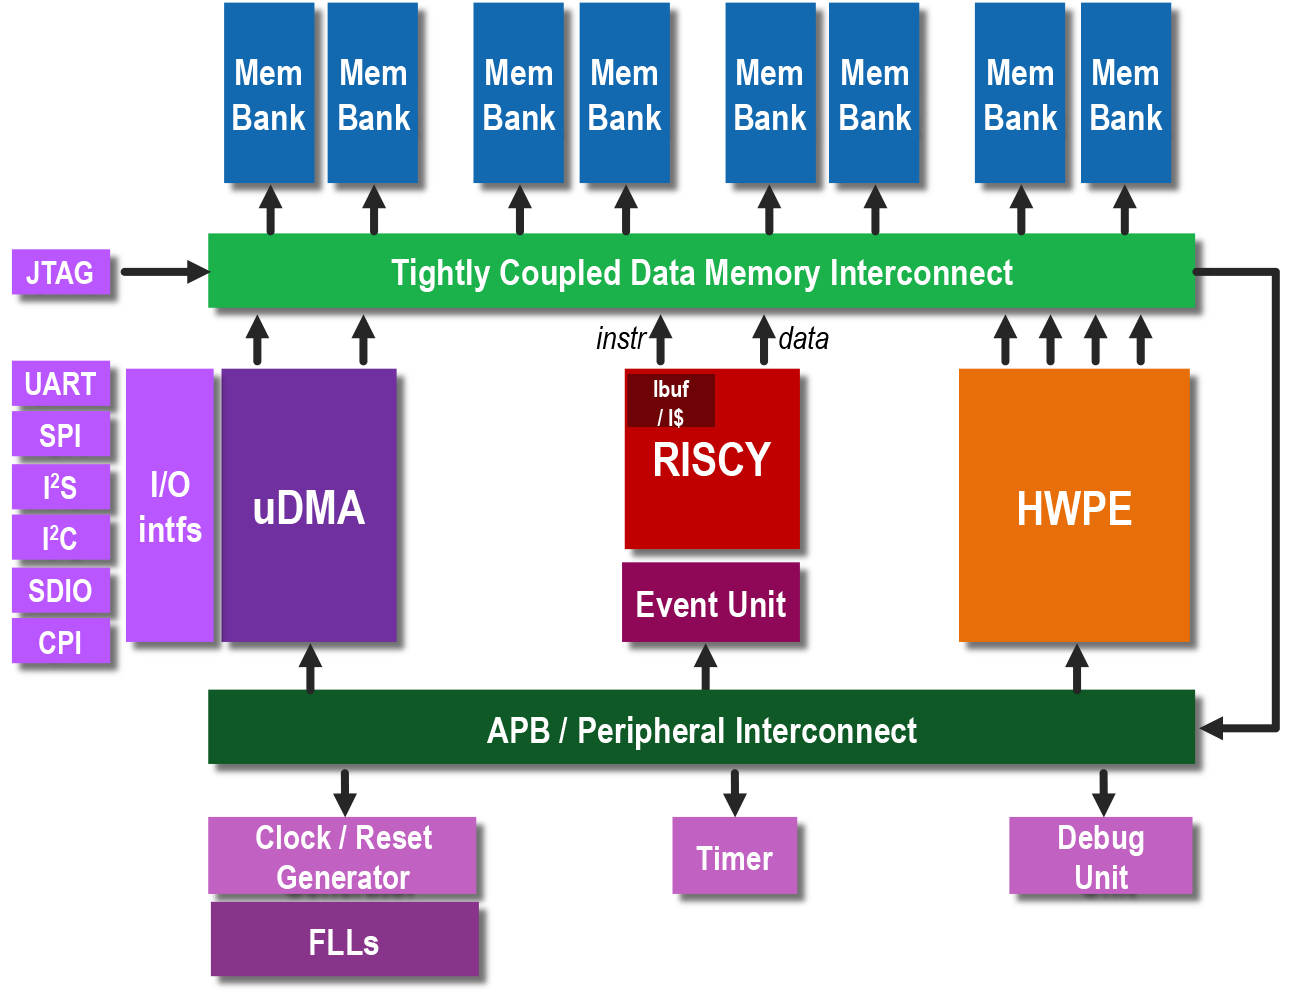
\includegraphics[width=0.7\linewidth]{images/congtrinhlienquan/pulpissimo_archi.png}
    \caption{Kiến trúc Pulpissimo}
    \label{fig:pulpissimo_archi}
\end{figure}

\subsection{Các đặc điểm kỹ thuật nổi bật}
PULPissimo bao gồm các thành phần chính sau:
\begin{itemize}
    \item Bộ xử lý chính: Hoặc bộ xử lý RI5CY hoặc bộ xử lý Ibex
    \item Hệ thống con uDMA: Hệ thống con đầu vào/đầu ra tự động để quản lý thiết bị ngoại vi hiệu quả
    \item Hệ thống con bộ nhớ: Bao gồm ROM khởi động và bộ nhớ L2
    \item Hệ thống sự kiện và ngắt: Bộ điều khiển ngắt đơn giản để quản lý các sự kiện hệ thống
    \item Thiết bị ngoại vi: Bao gồm SPI, I2S, giao diện camera, I2C, UART, Hyperbus và GPIO
    \item Bộ xử lý phần cứng (HWPE): Hỗ trợ các bộ tăng tốc phần cứng tùy chỉnh
\end{itemize}
\subsubsection{Lõi xử lý RI5CY/CV32E40P}
Trung tâm của Pulpissimo là nhân xử lý RI5CY (hiện nay được chuẩn hóa thành CV32E40P bởi OpenHW Group). 
Đây là một hiện thực hóa (implementation) của RISC-V với đường ống 4 tầng, được tối ưu hóa đặc biệt cho 
xử lý tín hiệu số (DSP).
Điểm đặc biệt của nhân này là việc hỗ trợ các mở rộng tập lệnh không tiêu chuẩn (Non-standard Extensions) 
giúp tăng tốc đáng kể các thuật toán AI:
\begin{itemize}
    \item \textbf{Hardware Loops:} Cho phép thực hiện các vòng lặp mà không tốn chu kỳ máy cho 
    việc kiểm tra điều kiện và rẽ nhánh.
    \item \textbf{SIMD (Single Instruction Multiple Data):} Hỗ trợ tính toán song song trên các 
    vector nhỏ (ví dụ: thực hiện 2 phép cộng 16-bit hoặc 4 phép cộng 8-bit trong 1 chu kỳ). 
    Đây là tính năng then chốt để xử lý dữ liệu lượng tử hóa (Quantized Data) trong mạng nơ-ron.
    \item \textbf{Bit Manipulation:} Các lệnh thao tác bit giúp tối ưu hóa việc đóng gói và giải nén 
    dữ liệu trọng số.
\end{itemize}

\subsubsection{Hệ thống bộ nhớ và uDMA}
Để giải quyết bài toán "nghẽn cổ chai" dữ liệu, Pulpissimo sử dụng bộ điều khiển truy cập bộ nhớ 
trực tiếp thông minh (micro-DMA hay uDMA). uDMA cho phép truyền dữ liệu trực tiếp từ các ngoại 
vi tốc độ cao (như Camera Interface, SPI) vào bộ nhớ nội (L2 Memory) mà không cần sự can thiệp 
của CPU. Cơ chế này giúp CPU có thể chuyển sang trạng thái ngủ (Sleep Mode) trong khi dữ liệu đang 
được thu thập, giúp tiết kiệm năng lượng tối đa .

\newpage
\section{Mạng nơ-ron Nhị phân (BNN)}

Trong nỗ lực giảm thiểu tài nguyên phần cứng cho các thiết bị biên, BNN nổi lên như một hướng 
nghiên cứu đột phá, đặc biệt phù hợp với cấu trúc của FPGA. Công trình nền tảng của Courbariaux 
và cộng sự \cite{bnn_courbariaux} đã chứng minh khả năng huấn luyện các mạng nơ-ron 
sâu với trọng số và tín hiệu kích hoạt bị ràng buộc ở hai mức giá trị.

\subsection{Cơ sở toán học và Nguyên lý hoạt động}

\subsubsection{Hàm nhị phân hóa (Binarization Function)}
Khác với các mạng CNN truyền thống sử dụng số thực 32-bit (FP32), BNN ép buộc các trọng số (Weights) 
và giá trị kích hoạt (Activations) về miền giá trị $\{+1, -1\}$. Courbariaux đề xuất hai phương pháp 
nhị phân hóa:
\begin{itemize}
    \item \textbf{Nhị phân hóa tất định (Deterministic Binarization):} Sử dụng hàm dấu (Sign function):
    \begin{equation}
        x^b = \text{Sign}(x) = \begin{cases} +1 & \text{if } x \geq 0 \\ -1 & \text{if } x < 0 \end{cases}
    \end{equation}
    Đây là phương pháp thường được sử dụng trong giai đoạn suy luận (Inference) trên phần cứng.
    \item \textbf{Nhị phân hóa ngẫu nhiên (Stochastic Binarization):} Sử dụng xác suất dựa trên 
    hàm sigmoid, thường dùng trong quá trình huấn luyện để tránh bị kẹt ở cực trị cục bộ, 
    tuy nhiên ít được áp dụng khi triển khai phần cứng do chi phí tính toán cao.
\end{itemize}

\subsubsection{Chiến lược huấn luyện với Straight-Through Estimator (STE)}
Thách thức lớn nhất khi huấn luyện BNN là hàm $\text{Sign}(x)$ không khả vi 
(đạo hàm bằng 0 ở hầu hết mọi nơi), khiến thuật toán lan truyền ngược (Backpropagation) không thể 
cập nhật trọng số.
Để giải quyết vấn đề này, Courbariaux áp dụng kỹ thuật \textbf{Straight-Through Estimator (STE)}. 
Trong quá trình lan truyền ngược, gradient được truyền xuyên qua hàm dấu mà không bị biến đổi 
(hoặc chỉ bị cắt bởi hàm Hard Tanh), coi như hàm dấu là hàm đồng nhất (Identity function) 
trong một khoảng nhất định:
\begin{equation}
    g_x \approx g_{x^b} \cdot \mathbf{1}_{|x| \le 1}
\end{equation}
Nhờ đó, mạng BNN có thể được huấn luyện "End-to-end" tương tự như các mạng CNN thông thường.

\subsection{Kiến trúc phần cứng trên FPGA}

Lợi thế cốt lõi của BNN nằm ở việc thay thế các phép toán đại số tuyến tính tốn kém bằng các phép toán 
logic bit-wise:

\begin{itemize}
    \item \textbf{Thay thế bộ nhân (Multiplier-less):} Phép nhân giữa một giá trị nhị phân 
    kích hoạt $a \in \{+1, -1\}$ và trọng số $w \in \{+1, -1\}$ có thể được mô hình hóa chính 
    xác bằng phép toán cổng \textbf{XNOR}:
    \begin{equation}
        a \cdot w \Leftrightarrow \neg(a \oplus w)
    \end{equation}
    Trên FPGA, một cổng XNOR tiêu tốn tài nguyên LUT không đáng kể so với một khối DSP48E2 dùng cho 
    phép nhân số thực.
    
    \item \textbf{Thay thế phép cộng (Accumulation):} Phép tích chập (Convolution) bao gồm việc tính 
    tổng các tích số. Trong BNN, thao tác này trở thành việc đếm số lượng bit 1 trong vector 
    kết quả XNOR, gọi là phép \textbf{Popcount} (Population Count). 
    \begin{equation}
        \mathbf{a} \cdot \mathbf{w} \approx 2 \cdot \text{popcount}(\text{xnor}(\mathbf{a}, 
        \mathbf{w})) - N
    \end{equation}
    (Với $N$ là độ dài vector).
\end{itemize}

\subsection{Hiệu quả tài nguyên và Giới hạn}
Theo kết quả thực nghiệm từ bài báo gốc, việc sử dụng BNN giúp giảm kích thước bộ nhớ xuống 
\textbf{32 lần} so với FP32, cho phép toàn bộ mô hình (hoặc các lớp lớn) nằm gọn trong bộ nhớ nội 
(Block RAM/UltraRAM) của FPGA. Điều này loại bỏ nút thắt cổ chai về băng thông bộ nhớ ngoài 
(Von Neumann bottleneck), giúp tăng tốc độ xử lý lên đáng kể.

\begin{figure}[!h]
    \centering
    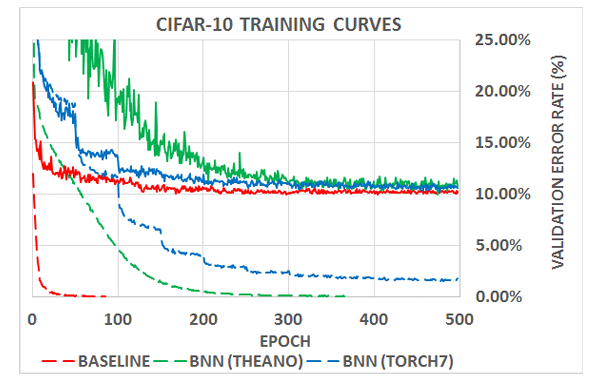
\includegraphics[width=0.8\linewidth]{images//congtrinhlienquan/bnn.png}
    \caption{Đường cong huấn luyện của mạng ConvNet trên tập dữ liệu CIFAR-10 tùy thuộc vào phương pháp.}
    \label{fig:placeholder}
\end{figure}

Tuy nhiên, BNN cũng bộc lộ hạn chế về độ chính xác (Accuracy Drop), đặc biệt với các bộ dữ liệu 
phức tạp như ImageNet. Do đó, trong đồ án này, chúng tôi tham khảo nguyên lý tối ưu phần cứng 
của BNN nhưng lựa chọn giải pháp \textbf{Lượng tử hóa 8-bit (INT8)} để đạt được sự cân bằng tối ưu 
giữa độ chính xác và hiệu năng trên nền tảng Kria KV260. Do đó, trong khuôn khổ đồ án này, 
nhóm nghiên cứu lựa chọn giải pháp lượng tử hóa điểm tĩnh (Fixed-point Quantization) 8-bit hoặc 16-bit 
để đảm bảo sự cân bằng tốt hơn giữa độ chính xác nhận dạng và hiệu năng phần cứng.


%=================================================================================
%=
%=================================================================================
\section{MobileNet}
\label{sec:mobilenet}

MobileNet là lớp các mô hình hiệu quả được Google giới thiệu nhằm phục vụ các ứng dụng thị giác máy tính 
trên thiết bị di động và nhúng. Kiến trúc này dựa trên luồng xử lý tinh gọn, sử dụng tích chập tách biệt 
theo chiều sâu (depthwise separable convolutions) để xây dựng các mạng nơ-ron sâu 
nhưng nhẹ \cite{mobilenet_v1}.

\subsection{Tích chập Tách biệt theo Chiều sâu (Depthwise Separable Convolution)}
Cốt lõi của MobileNet là thay thế cấu trúc tích chập tiêu chuẩn bằng tích chập tách biệt. 
Một lớp tích chập tiêu chuẩn lọc và kết hợp các đặc trưng đầu vào thành tập hợp đầu ra mới 
trong một bước duy nhất. Ngược lại, tích chập tách biệt chia quá trình này thành 
hai lớp riêng biệt:
\begin{enumerate}
    \item \textbf{Depthwise Convolution:} Áp dụng một bộ lọc duy nhất cho mỗi kênh đầu vào 
    để lọc đặc trưng.
    \item \textbf{Pointwise Convolution:} Sử dụng tích chập $1 \times 1$ để tổ hợp tuyến 
    tính các đầu ra từ lớp depthwise.
\end{enumerate}

Xét một lớp tích chập với đầu vào kích thước $D_F \times D_F \times M$ và đầu ra $D_F 
\times D_F \times N$, sử dụng kernel $D_K \times D_K$. 
Chi phí tính toán của tích chập tiêu chuẩn là:
\begin{equation}
    C_{std} = D_K \cdot D_K \cdot M \cdot N \cdot D_F \cdot D_F
\end{equation}

Trong khi đó, chi phí của tích chập tách biệt theo chiều sâu là tổng của hai bước 
(depthwise và pointwise):
\begin{equation}
    C_{sep} = D_K \cdot D_K \cdot M \cdot D_F \cdot D_F + M \cdot N \cdot D_F \cdot D_F
\end{equation}

Tỷ lệ giảm khối lượng tính toán đạt được là:
\begin{equation}
    \frac{C_{sep}}{C_{std}} = \frac{1}{N} + \frac{1}{D_K^2}
\end{equation}
Với MobileNet sử dụng kernel $3 \times 3$, kiến trúc này giúp giảm khối lượng tính toán 
từ 8 đến 9 lần so 
với tích chập truyền thống với mức giảm độ chính xác không đáng kể.

\begin{figure}[!h]
    \centering
    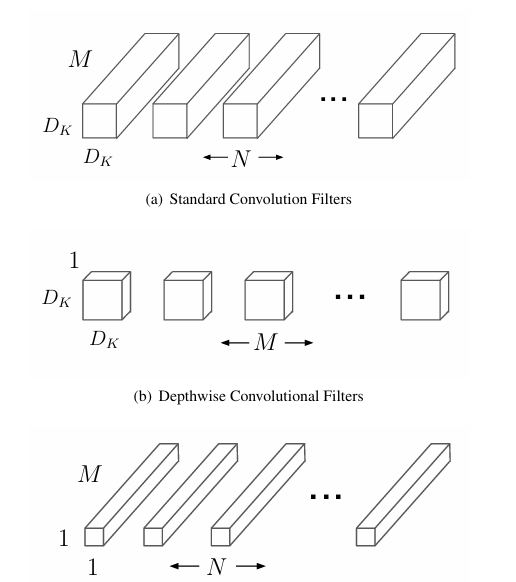
\includegraphics[width=0.7\linewidth]{images/congtrinhlienquan/mobile.png}
    \caption{Kiến trúc của MobileNet với các lớp depthwise và pointwise.}
    \label{fig:mobilenet}
\end{figure}

\subsection{Kiến trúc và Tham số Tinh chỉnh (Hyperparameters)}
\subsubsection{Cấu trúc mạng}
MobileNet bao gồm 28 lớp nếu tính riêng biệt các lớp depthwise và pointwise. Một điểm đặc biệt trong 
thiết kế là 95\% thời gian tính toán của mạng tập trung vào các lớp tích chập $1 \times 1$ (Pointwise). 
Điều này cực kỳ có lợi cho phần cứng FPGA vì tích chập $1 \times 1$ không yêu cầu sắp xếp lại 
bộ nhớ (im2col) và có thể được hiện thực hóa trực tiếp bằng các thuật toán nhân ma trận (GEMM) 
được tối ưu hóa cao.

Tất cả các lớp trong MobileNet đều được theo sau bởi chuẩn hóa theo lô (Batch Normalization) 
và hàm kích hoạt phi tuyến ReLU, ngoại trừ lớp kết nối đầy đủ cuối cùng đưa vào Softmax.

\begin{figure}[!h]
    \centering
    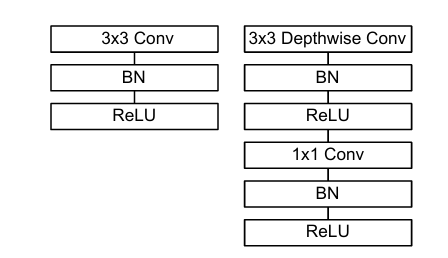
\includegraphics[width=0.8\linewidth]{images/congtrinhlienquan/mobilenet_arch.png}
    \caption{Cấu trúc chi tiết của MobileNetV1}
    \label{fig:mobilenet_archi}
\end{figure}

\newpage
\subsubsection{Các bộ nhân độ rộng và độ phân giải}
Để tùy biến mô hình cho các ràng buộc tài nguyên cụ thể, MobileNet giới thiệu hai tham số siêu hình 
đơn giản:

\begin{itemize}
    \item \textbf{Width Multiplier ($\alpha$):} Có vai trò làm "mỏng" mạng một cách 
    đồng nhất tại mỗi lớp. 
    Với một hệ số $\alpha \in (0, 1]$, số lượng kênh đầu vào $M$ trở thành $\alpha M$ 
    và đầu ra $N$ trở thành $\alpha N$. Chi phí tính toán và số lượng tham số giảm 
    theo hàm bậc hai, xấp xỉ $\alpha^2$[cite: 172].
    \item \textbf{Resolution Multiplier ($\rho$):} Được áp dụng lên hình ảnh đầu vào, 
    làm giảm biểu diễn nội tại của mọi lớp tiếp theo. Hệ số $\rho \in (0, 1]$ giúp giảm 
    chi phí tính toán theo tỷ lệ $\rho^2$.
\end{itemize}

\subsection{Hiệu quả Thực nghiệm}
Các thử nghiệm trên tập dữ liệu ImageNet cho thấy MobileNet đạt hiệu quả vượt trội so với 
các mô hình phổ biến khác.
\begin{itemize}
    \item So với \textbf{VGG16}: MobileNet đạt độ chính xác gần tương đương nhưng có kích 
    thước nhỏ hơn 32 lần và khối lượng tính toán ít hơn 27 lần.
    \item So với \textbf{GoogleNet}: MobileNet chính xác hơn, nhỏ hơn và tính toán ít hơn 2.5 lần.
    \item Khả năng ứng dụng rộng rãi: Ngoài phân loại ảnh, MobileNet còn chứng minh hiệu 
    quả cao trong các tác vụ phát hiện vật thể (Object Detection), phân loại chi tiết 
    (Fine-grain classification), và định vị địa lý quy mô lớn.
\end{itemize}


%=================================================================================
%=
%=================================================================================

\section{Lượng tử hóa và Huấn luyện mạng nơ-ron (Quantization \& Training)}
\label{sec:quantization_theory}

Trong các hệ thống học sâu truyền thống, việc huấn luyện và suy luận thường được 
thực hiện trên định dạng số thực dấu phẩy động 32-bit (Float32) để đảm bảo độ chính xác cao nhất. Tuy nhiên, trên các thiết bị biên (Edge Devices) với tài nguyên hạn chế như FPGA hay vi xử lý nhúng RISC-V, các phép toán số thực tiêu tốn quá nhiều tài nguyên phần cứng và năng lượng.

Để giải quyết vấn đề này, đồ án áp dụng phương pháp lượng tử hóa số nguyên 
được đề xuất bởi \textit{Jacob et al.} (Google) trong công trình 
\textit{"Quantization and Training of Neural Networks for Efficient 
Integer-Arithmetic-Only Inference"} \cite{jacob2018quantization}.

\begin{figure}[!h]
    \centering
    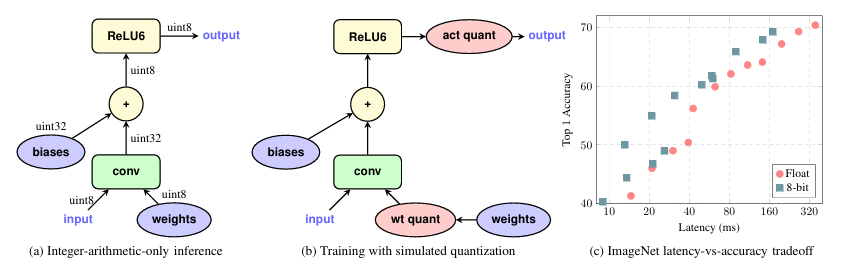
\includegraphics[width=1\linewidth]{images/congtrinhlienquan/quanti.png}
    \caption{Quy trình lượng tử hóa và huấn luyện mạng nơ-ron theo Jacob et al.}
    \label{fig:quantization_process}
\end{figure}

\subsection{Cơ chế Lượng tử hóa Affine (Affine Quantization Scheme)}
Khác với các phương pháp lượng tử hóa logarit hay nhị phân, phương pháp của Jacob et al. sử dụng ánh xạ tuyến tính (Affine mapping) để chuyển đổi giữa giá trị thực ($r$) và giá trị nguyên 8-bit ($q$). Công thức ánh xạ được định nghĩa như sau:

\begin{equation}
    r = S \times (q - Z)
\end{equation}

Trong đó:
\begin{itemize}
    \item $r$ (Real value): Giá trị thực cần biểu diễn.
    \item $q$ (Quantized value): Giá trị nguyên 8-bit ($q \in [0, 255]$ hoặc $[-128, 127]$).
    \item $S$ (Scale factor): Hằng số tỉ lệ (dạng Float32 dương), xác định bước nhảy của lượng tử hóa.
    \item $Z$ (Zero-point): Giá trị nguyên đóng vai trò là điểm "0" của số thực. Điều này cho phép biểu diễn chính xác giá trị 0 thực tế (thường xuất hiện trong Padding hoặc ReLU) bằng một số nguyên, giúp duy trì độ chính xác của mạng.
\end{itemize}

Từ công thức trên, quá trình nhân chập (Convolution) giữa đầu vào $x$ và trọng số $w$ có thể được viết lại hoàn toàn dưới dạng số nguyên:

\begin{equation}
    y = \sum (x \times w) \approx S_y \left( \sum (q_x - Z_x)(q_w - Z_w) + Z_y \right)
\end{equation}

\subsection{Suy luận chỉ dùng số học nguyên (Integer-Arithmetic-Only Inference)}
Điểm đột phá trong nghiên cứu của Jacob et al. là kỹ thuật xử lý tham số $S$ (Scale). Mặc dù $S$ là số thực, nhưng trong quá trình suy luận, tích của các Scale ($M = S_x S_w / S_y$) được xấp xỉ bằng một phép nhân số nguyên và phép dịch bit (Bit-shift):

\begin{equation}
    M \approx 2^{-n} \times M_0 \quad (\text{với } M_0 \text{ là số nguyên cố định})
\end{equation}

Kỹ thuật này cho phép loại bỏ hoàn toàn khối xử lý số thực (FPU) khỏi phần cứng. 
Mọi phép tính từ tích chập, cộng bias đến hàm kích hoạt đều được thực hiện bằng 
các đơn vị số học nguyên (ALU Integer) và các bộ dịch bit.

\chapter{Kiến trúc hệ thống đề xuất}

\section{Tổng quan kiến trúc hệ thống}

Hệ thống Edge-AI được thiết kế dựa trên kiến trúc không đồng nhất 
(Heterogeneous Architecture) của nền tảng Zynq UltraScale+ MPSoC trên bo mạch Kria KV260. 
Thiết kế tận dụng mô hình đồng thiết kế phần cứng/phần mềm (Hardware/Software Co-design)
 để tối ưu hóa hiệu năng xử lý.

\begin{figure}[!h]
\centering
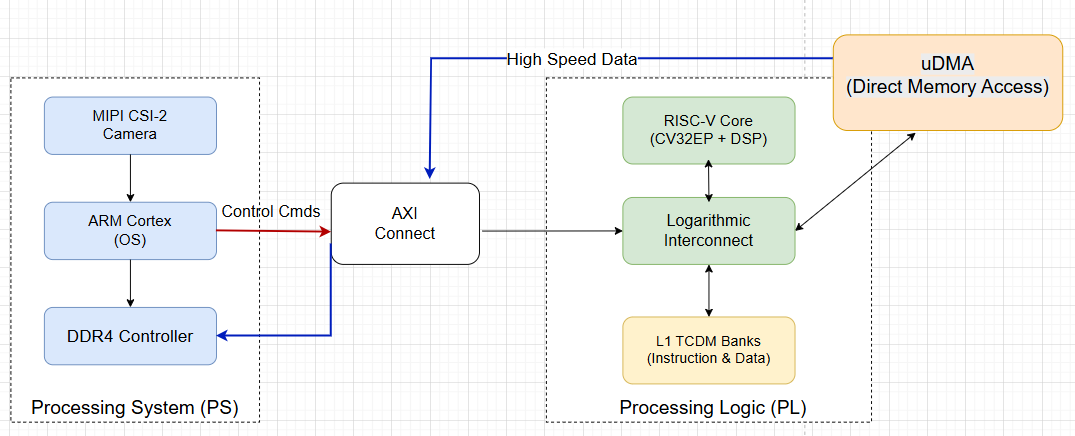
\includegraphics[width=1\textwidth]{images/design/arch.png}
\caption{Kiến trúc hệ thống tổng quan}
\label{fig:proposed_architecture}
\end{figure}

Mô hình tổng thể được chia thành hai miền xử lý chính:
\begin{itemize}
    \item Processing System
    \item Khối Cầu nối
    \item Programmable Logic
\end{itemize}

Như thể hiện tại Hình \ref{fig:proposed_architecture}, hệ thống được phân chia thành ba miền xử lý chính với các vai trò chuyên biệt:

\begin{itemize}
    \item \textbf{Phân hệ Xử lý (Processing System - PS):} 
    Đóng vai trò là khối điều khiển trung tâm (Host), hoạt động trên nền tảng vi xử lý ARM Cortex-A53 lõi tứ. PS chịu trách nhiệm:
    \begin{itemize}
        \item Quản lý tài nguyên hệ thống và khởi chạy quy trình boot.
        \item Giao tiếp với các ngoại vi tiêu chuẩn như Camera (qua giao diện MIPI CSI-2) và Màn hình.
        \item Thực hiện các bước tiền xử lý hình ảnh (Preprocessing) và quản lý bộ nhớ đệm dữ liệu (Data Buffering) trên DDR4.
    \end{itemize}

    \item \textbf{Khối Giao tiếp Liên kết (Interconnect Fabric):} 
    Đóng vai trò là cầu nối dữ liệu tốc độ cao, sử dụng giao thức chuẩn công nghiệp AMBA AXI4. Khối này bao gồm các bộ chuyển mạch thông minh (AXI SmartConnect) để:
    \begin{itemize}
        \item Phân tách luồng điều khiển (Control Plane) băng thông thấp và luồng dữ liệu (Data Plane) băng thông cao.
        \item Đảm bảo đồng bộ hóa giữa hai miền xung nhịp khác nhau của PS và PL.
        \item Cho phép truy cập bộ nhớ chia sẻ (Shared Memory) một cách trong suốt giữa các vi xử lý.
    \end{itemize}

    \item \textbf{Phân hệ Logic Khả trình (Programmable Logic - PL):} 
    Đóng vai trò là bộ tăng tốc tính toán (Accelerator). Tại đây, tài nguyên FPGA được cấu hình để triển khai một Hệ thống trên Chip (SoC) con, bao gồm:
    \begin{itemize}
        \item \textbf{Lõi vi xử lý mềm RISC-V (PULP Subsystem):} Điều phối luồng thực thi thuật toán AI.
        \item \textbf{Bộ tăng tốc phần cứng (CNN Accelerator):} Thực hiện các phép toán tích chập chuyên sâu.
        \item \textbf{Cơ chế truy cập bộ nhớ trực tiếp (uDMA):} Tối ưu hóa việc di chuyển dữ liệu ảnh mà không làm gián đoạn CPU.
    \end{itemize}
\end{itemize}

Sự kết hợp chặt chẽ giữa ba thành phần này cho phép hệ thống hoạt động theo cơ chế đường ống (Pipelining), đảm bảo khả năng xử lý hình ảnh thời gian thực với độ trễ thấp nhất.

%=======================================================================
\newpage
\section{Thiết kế Processing System}

Đây là phần cứng có sẵn (Hard-core) trên chip Zynq UltraScale+ của board Kria KV260.
\begin{itemize}
    \item ARM Cortex-A53: Đóng vai trò là CPU chủ (Host). Nó có thểchạy hệ điều hành (Linux hoặc Bare-metal) 
để quản lý toàn bộ hệ thống. Nhiệm vụ của nó là giao tiếp với Camera (qua cổng MIPI), 
nhận ảnh, tiền xử lý (resize, crop) và lưu trữ ảnh vào bộ nhớ lớn.
    \item DDR4 Controller (Shared Memory): Đây là kho chứa dữ liệu chung. Vì bộ nhớ trong của RISC-V 
rất nhỏ (chỉ vài chục KB), toàn bộ dữ liệu ảnh đầu vào (Image Buffer) phải được lưu ở đây 
(4GB RAM của Kria).
\end{itemize}

PS đóng vai trò "Master" điều phối, gửi lệnh "Bắt đầu" (Start) cho khối PL 
khi đã có dữ liệu ảnh sẵn sàng.

\subsection{Sơ đồ cấu hình khối Zynq UltraScale+ (PS Block Design)}

\begin{figure}[!h]
    \centering
    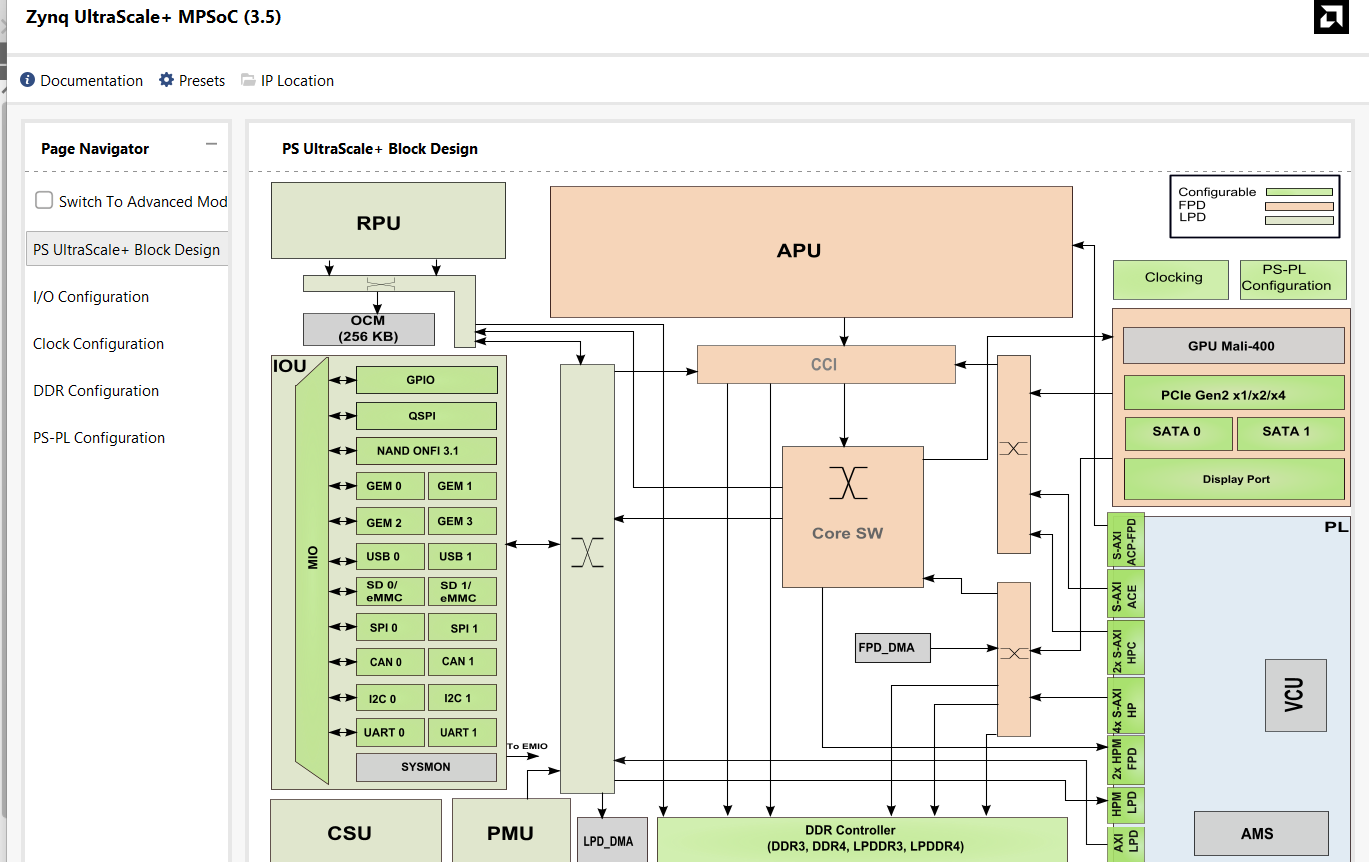
\includegraphics[width=1\textwidth]{images/design/zynq.png}  
    \caption{Sơ đồ cấu hình khối Zynq UltraScale+ MPSoC trên Vivado.}
    \label{fig:ps_block_design}
\end{figure}

\subsection{Cấu hình chi tiết các phân hệ}

\subsubsection{Khối xử lý ứng dụng (APU Configuration)}
Trung tâm của PS là cụm vi xử lý Quad-core ARM Cortex-A53 hoạt động ở tần số 1.2 GHz. Trong thiết kế này, APU được cấu hình để:
\begin{itemize}
    \item \textbf{Chế độ hoạt động:} Chạy hệ điều hành PetaLinux (dựa trên Yocto Project) để tận dụng các driver có sẵn cho Camera MIPI và ngăn xếp mạng (Network Stack).
    \item \textbf{Quản lý Boot:} Sử dụng giao diện SD Card (SD1) kết nối với các chân MIO để nạp bitstream cho FPGA và khởi động hệ thống.
\end{itemize}

\subsubsection{Cấu hình Giao diện Bộ nhớ (DDR Configuration)}
Bộ điều khiển DDR4 (DDRC) được kích hoạt để quản lý 4GB RAM tích hợp trên Kria SOM. Cấu hình này rất quan trọng vì nó đóng vai trò là "Shared Memory" cho cả hệ thống:
\begin{itemize}
    \item \textbf{Data Width:} 64-bit (hỗ trợ băng thông cao).
    \item \textbf{AXI Port QoS:} Cổng S\_AXI\_HP0 được ưu tiên mức Quality of Service (QoS) cao để đảm bảo uDMA không bị nghẽn khi ghi dữ liệu ảnh, tránh hiện tượng rớt khung hình (frame drop).
\end{itemize}

\subsubsection{Cấu hình Giao diện PS-PL (Interface Configuration)}
Để kết nối với miền Logic khả trình (nơi chứa RISC-V và Accelerator), hai cổng giao tiếp AXI quan trọng được kích hoạt:

\begin{enumerate}
    \item \textbf{M\_AXI\_HPM0\_FPD (Master):}
    \begin{itemize}
        \item \textit{Chức năng:} Cổng Master hiệu năng cao miền công suất thấp (Full Power Domain).
        \item \textit{Nhiệm vụ:} Dùng để CPU ARM gửi tín hiệu điều khiển, cấu hình thanh ghi và nạp firmware vào bộ nhớ lệnh của RISC-V.
        \item \textit{Độ rộng:} 32-bit (phù hợp với bus AXI-Lite).
    \end{itemize}
    
    \item \textbf{S\_AXI\_HP0\_FPD (Slave):}
    \begin{itemize}
        \item \textit{Chức năng:} Cổng Slave hiệu năng cao (High Performance).
        \item \textit{Nhiệm vụ:} Cho phép các Master bên phía FPGA (cụ thể là uDMA) truy cập trực tiếp vào RAM DDR4.
        \item \textit{Độ rộng:} 128-bit (để tối đa hóa tốc độ truyền tải ảnh).
    \end{itemize}
\end{enumerate}

\subsubsection{Cấu hình Xung nhịp (Clock Configuration)}
Khối PS cung cấp nguồn xung nhịp tham chiếu cho toàn bộ logic bên phía PL 
thông qua chân \texttt{pl\_clk0}. Tần số được thiết lập là \textbf{100 MHz}, 
đảm bảo sự cân bằng giữa tốc độ xử lý của nhân RISC-V và mức tiêu thụ năng lượng.

%=========================================================
\newpage
\section{Thiết kế Hệ thống Giao tiếp và Bộ nhớ (Interconnect \& Memory Hierarchy)}
\label{sec:interconnect_design}

Trong kiến trúc SoC dị thể, hiệu năng của hệ thống không chỉ phụ thuộc vào tốc độ xử lý của từng nhân (Core) mà còn phụ thuộc vào băng thông và độ trễ của hệ thống kết nối. Mục này trình bày thiết kế chi tiết mạng lưới giao tiếp giữa PS và PL, cùng với quy hoạch không gian bộ nhớ chung.

\begin{figure}[h]
    \centering
    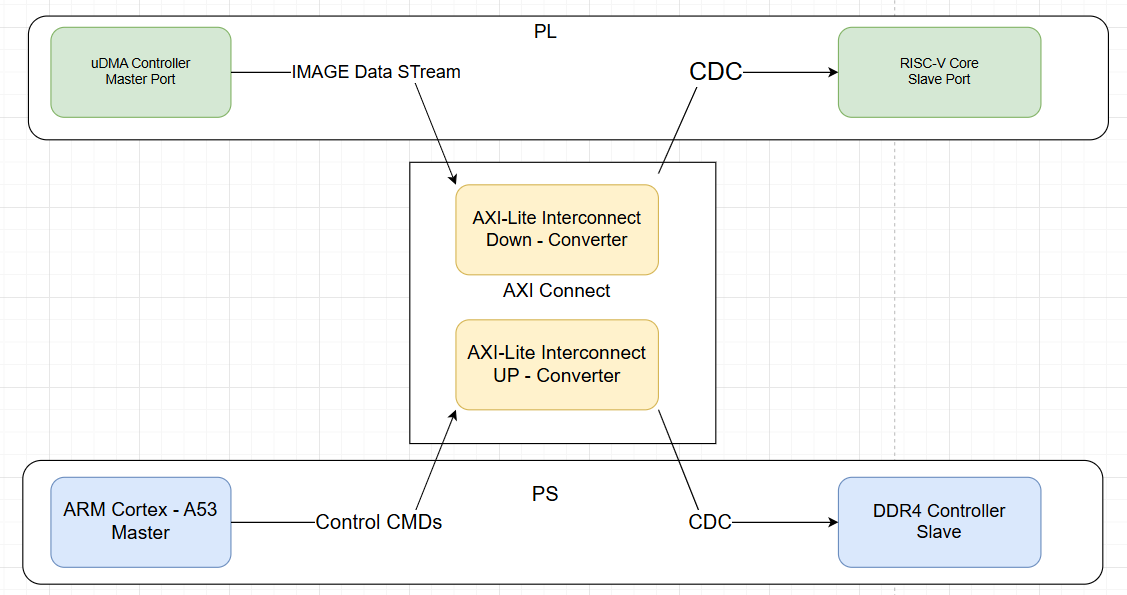
\includegraphics[width=1\textwidth]{images/design/axi_arch.png}  
    \caption{Sơ đồ khối hệ thống giao tiếp AXI giữa PS và PL.}
    \label{fig:axi_interconnect}
\end{figure}


\subsection{Cơ chế AXI SmartConnect (PS-PL Bridge)}
Để kết nối miền xử lý ứng dụng (PS) hoạt động ở tần số cao và miền logic khả trình (PL) hoạt động ở tần số thấp, hệ thống sử dụng khối IP **AXI SmartConnect**. Đây không chỉ là dây dẫn đơn thuần mà là một ma trận chuyển mạch thông minh (Switch Fabric) đảm nhiệm ba chức năng:
\begin{itemize}
    \item \textbf{Clock Domain Crossing (CDC):} Đồng bộ hóa tín hiệu giữa miền xung nhịp PS (1.2 GHz) và miền PL (100 MHz) bằng các bộ đệm FIFO bất đồng bộ, đảm bảo không xảy ra lỗi Metastability.
    \item \textbf{Width Conversion:} Chuyển đổi độ rộng dữ liệu tự động giữa bus hệ thống 128-bit (phía DDR) và bus ngoại vi 32-bit (phía RISC-V).
    \item \textbf{Arbitration:} Phân giải tranh chấp khi nhiều Master cùng truy cập bộ nhớ.
\end{itemize}

Hệ thống được thiết kế với hai kênh giao tiếp vật lý tách biệt:

\subsubsection{Kênh Điều khiển (Control Path - AXI4-Lite)}
Đây là tuyến giao tiếp từ \textbf{Master (ARM Cortex-A53)} đến \textbf{Slave (PULP Subsystem)}.
\begin{itemize}
    \item \textbf{Giao thức:} AXI4-Lite 32-bit. Đây là phiên bản rút gọn của AXI4, không hỗ trợ truyền tải dạng Burst.
    \item \textbf{Mục đích:} Tối ưu hóa cho các giao dịch đơn lẻ, độ trễ thấp.
    \item \textbf{Chức năng:} Dùng để CPU ARM thực hiện các tác vụ quản trị như:
    \begin{itemize}
        \item Cấu hình thanh ghi điều khiển của bộ tăng tốc CNN (Trọng số, Bias, Kích thước ảnh).
        \item Gửi tín hiệu kích hoạt (Trigger) quá trình suy luận.
        \item Reset mềm (Soft-reset) khối PL trong trường hợp treo hệ thống.
    \end{itemize}
\end{itemize}

\subsubsection{Kênh Dữ liệu (Data Path - AXI4-Full)}
Đây là tuyến giao tiếp từ \textbf{Master (uDMA Controller)} đến \textbf{Slave (DDR4 Controller)}.
\begin{itemize}
    \item \textbf{Giao thức:} AXI4-Full 128-bit.
    \item \textbf{Mục đích:} Tối ưu hóa băng thông (Throughput).
    \item \textbf{Chức năng:} Hỗ trợ cơ chế \textit{Burst Transaction}, cho phép uDMA đọc/ghi liên tiếp tới 256 gói dữ liệu chỉ với một địa chỉ bắt đầu. Điều này cực kỳ quan trọng để đảm bảo cung cấp đủ dữ liệu pixel cho mạng MobileNet hoạt động thời gian thực (Real-time).
\end{itemize}

\subsection{Quy hoạch không gian bộ nhớ (System Memory Map)}
Do RISC-V Soft-core sử dụng kiến trúc bộ nhớ phẳng (Flat Memory Model) 32-bit, việc phân chia địa chỉ phải được thiết kế cẩn trọng để map chính xác với địa chỉ vật lý của hệ thống Zynq.

Bảng \ref{tab:memory_map} mô tả bản đồ bộ nhớ từ góc nhìn của vi xử lý RISC-V:

\begin{table}[h]
\centering
\caption{Bản đồ bộ nhớ hệ thống (System Memory Map)}
\label{tab:memory_map}
\begin{tabular}{|l|l|l|p{5cm}|}
\hline
\textbf{Vùng nhớ} & \textbf{Địa chỉ (Base)} & \textbf{Kích thước} & \textbf{Chức năng chi tiết} \\ \hline
\texttt{INSTR\_RAM} & \texttt{0x0000\_0000} & 64 KB & Bộ nhớ chứa Firmware. Khi Reset, RISC-V sẽ trỏ PC (Program Counter) vào đây. \\ \hline
\texttt{DATA\_RAM} & \texttt{0x0010\_0000} & 64 KB & Vùng nhớ TCDM cục bộ, chứa Stack, Heap và biến cục bộ. Truy cập trong 1 chu kỳ. \\ \hline
\texttt{PERIPHERAL} & \texttt{0x1A10\_0000} & 4 KB & Vùng thanh ghi ngoại vi (MMIO) để điều khiển Timer, Event Unit và uDMA. \\ \hline
\textbf{\texttt{SHARED\_DDR}} & \textbf{\texttt{0x4000\_0000}} & \textbf{16 MB} & \textbf{Bộ nhớ chia sẻ (Shared Memory).} Được ánh xạ trực tiếp từ DDR4 của Zynq. Chứa Frame Buffer ảnh đầu vào và Output Tensor. \\ \hline
\texttt{MAILBOX} & \texttt{0xA000\_0000} & 4 KB & \textbf{Giao tiếp liên nhân (IPC).} Chứa các cờ hiệu (Semaphores) để đồng bộ trạng thái giữa ARM và RISC-V. \\ \hline
\end{tabular}
\end{table}

\subsubsection{Cơ chế Đồng bộ hóa (Mailbox Mechanism)}
Để tránh xung đột khi hai vi xử lý cùng truy cập vùng \texttt{SHARED\_DDR}, cơ chế Mailbox hoạt động như sau:
\begin{enumerate}
    \item \textbf{ARM:} Sau khi ghi ảnh vào DDR, ARM ghi giá trị \texttt{0x1} vào thanh ghi Mailbox để báo hiệu "Data Ready".
    \item \textbf{RISC-V:} Liên tục kiểm tra (Polling) hoặc nhận ngắt từ Mailbox. Khi thấy \texttt{0x1}, nó bắt đầu xử lý và ghi đè giá trị \texttt{0x2} ("Processing").
    \item \textbf{RISC-V:} Khi xử lý xong, ghi giá trị \texttt{0x3} ("Done").
    \item \textbf{ARM:} Đọc thấy \texttt{0x3}, lấy kết quả và reset Mailbox về \texttt{0x0}.
\end{enumerate}


%=============================================
%
%=============================================
\newpage
\section{Thiết kế Programmable Logic}
\label{sec:pl_design}

Logic Khả trình (PL) được thiết kế như một Hệ thống trên Chip (SoC) thu nhỏ hoạt động độc lập, dựa trên kiến trúc mở PULPissimo. Mục tiêu của phân hệ này là tạo ra một môi trường tính toán hiệu năng cao, độ trễ thấp để thực thi các tác vụ điều khiển và tăng tốc AI, giảm tải cho vi xử lý chính ARM.

\subsection{Kiến trúc tổng thể Phân hệ PULP (PULP Subsystem)}
Hình \ref{fig:pulp_arch} trình bày sơ đồ kiến trúc chi tiết của khối PL. Thiết kế bao gồm ba thành phần cốt lõi: Lõi xử lý RISC-V, Hệ thống bộ nhớ TCDM phân tán, và Bộ điều khiển uDMA, được kết nối với nhau thông qua một mạng lưới giao tiếp băng thông rộng (Logarithmic Interconnect).

\begin{figure}[h]
    \centering
    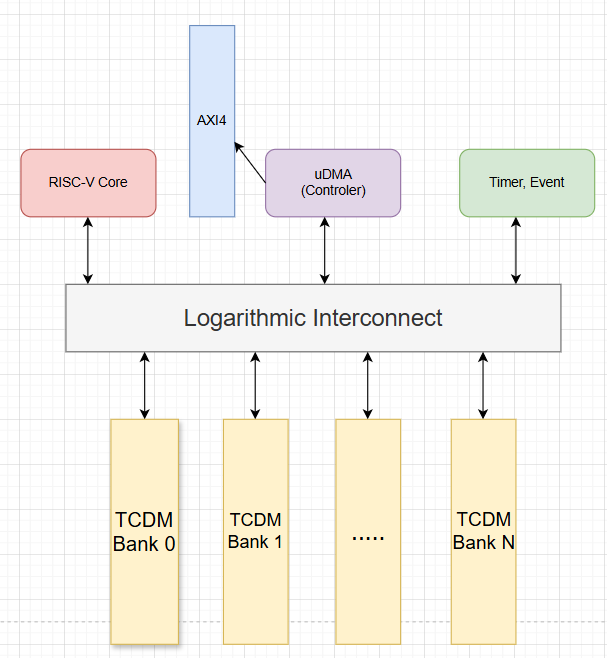
\includegraphics[width=0.8\textwidth]{images/design/pulp_arch.png}  
    \caption{Sơ đồ kiến trúc nội bộ của Phân hệ PULP trên FPGA.}
    \label{fig:pulp_arch}
\end{figure}

\subsection{Cấu hình Nhân Vi xử lý (RISC-V Core Configuration)}
Trung tâm điều khiển của PL là lõi IP RISC-V (dựa trên nhân CV32E40P). Lõi này được tham số hóa trước khi tổng hợp (Synthesis) để đạt sự cân bằng tối ưu giữa tài nguyên FPGA (LUTs) và hiệu năng tính toán:

\begin{table}[h]
\centering
\caption{Thông số cấu hình RISC-V Soft-core}
\label{tab:riscv_config}
\begin{tabular}{|l|l|p{6cm}|}
\hline
\textbf{Tham số} & \textbf{Giá trị} & \textbf{Ý nghĩa thiết kế} \\ \hline
Architecture & RV32IMCXpulp & Hỗ trợ tập lệnh nhân (M), nén (C) và mở rộng DSP/SIMD (Xpulp) cho AI. \\ \hline
Pipeline Stages & 4 & Đủ sâu để đạt tần số 100MHz, đủ ngắn để giảm độ trễ rẽ nhánh. \\ \hline
FPU & Disabled & Không sử dụng bộ xử lý dấu phẩy động để tiết kiệm diện tích (MobileNet đã được lượng tử hóa sang INT8). \\ \hline
Instruction Cache & 4 KB & Kiểu Direct Mapped, giúp CPU nạp lệnh nhanh mà không cần truy cập RAM ngoài liên tục. \\ \hline
Boot Address & \texttt{0x1A00\_0000} & Vị trí vector ngắt khởi động, trỏ tới vùng nhớ ROM khởi tạo. \\ \hline
\end{tabular}
\end{table}

\subsection{Hệ thống Bộ nhớ TCDM và Interconnect}
Điểm yếu chí tử của các hệ thống đa vi xử lý là hiện tượng tranh chấp bộ nhớ (Memory Contention). Thiết kế này giải quyết triệt để vấn đề trên bằng kiến trúc TCDM (Tightly Coupled Data Memory).

\subsubsection{Tổ chức Bộ nhớ Đan xen (Interleaved Memory Banking)}
Thay vì sử dụng một khối Block RAM khổng lồ đơn nhất (64KB), bộ nhớ TCDM được chia nhỏ thành \textbf{16 ngân hàng (Banks)}, mỗi ngân hàng có dung lượng 4KB.
\begin{itemize}
    \item \textbf{Nguyên lý:} Các địa chỉ liên tiếp nhau ($Addr, Addr+4, Addr+8...$) được lưu trữ lần lượt trên các Bank khác nhau ($Bank_0, Bank_1, Bank_2...$).
    \item \textbf{Lợi ích:} Cho phép truy cập song song. Ví dụ: RISC-V Core có thể đọc dữ liệu tại địa chỉ $A$ (nằm ở Bank 0) cùng lúc uDMA ghi dữ liệu vào địa chỉ $B$ (nằm ở Bank 1) mà không hề xảy ra xung đột.
\end{itemize}

\subsubsection{Logarithmic Interconnect}
Kết nối giữa các Master (Core, uDMA) và các Slave (Memory Banks) không phải là một Bus tuyến tính mà là một \textbf{Ma trận chuyển mạch (Switch Matrix)}.
\begin{itemize}
    \item Mạng lưới này có độ trễ cực thấp (chỉ 1 chu kỳ xung nhịp).
    \item Đảm bảo băng thông cực đại: Tổng băng thông nội bộ có thể đạt tới $N \times 32$-bit/cycle (với N là số lượng Bank).
\end{itemize}

\subsection{Cơ chế Truy cập Bộ nhớ Trực tiếp (uDMA)}
Để giải phóng CPU khỏi tác vụ sao chép dữ liệu nhàm chán, một bộ điều khiển uDMA (Micro-DMA) chuyên dụng được tích hợp:
\begin{itemize}
    \item \textbf{Chức năng:} uDMA đóng vai trò cầu nối giữa các ngoại vi tốc độ cao (như AXI4 port nối tới DDR4, SPI, Camera) và bộ nhớ TCDM.
    \item \textbf{Double Buffering:} uDMA hỗ trợ cấu hình hai vùng đệm (Buffer A và Buffer B). Khi đang xử lý dữ liệu ở Buffer A, uDMA sẽ tự động tải dữ liệu mới vào Buffer B trong nền (Background).
    \item \textbf{Kết nối với Accelerator:} uDMA cung cấp một luồng dữ liệu liên tục (Stream) cho khối tăng tốc CNN thông qua giao diện AXI-Stream, đảm bảo bộ tăng tốc luôn có dữ liệu để tính toán (tránh hiện tượng Starvation).
\end{itemize}

%=============================================================
\newpage
\section{Thiết kế Khối Tăng tốc phần cứng (CNN Accelerator)}
Nằm trong PL, khối tăng tốc CNN được thiết kế để thực hiện các phép toán tích chập
một cách song song và hiệu quả. Thiết kế này bao gồm các thành phần chính \cite{fpga2}
\label{sec:cnn_accelerator}

Đây là thành phần cốt lõi quyết định hiệu năng của toàn bộ hệ thống Edge-AI. 
Để đáp ứng yêu cầu tính toán thời gian thực của mạng MobileNetV1, nhóm thực hiện thiết kế một bộ tăng tốc phần cứng chuyên dụng (Domain-Specific Architecture - DSA) được tích hợp trong miền Logic khả trình (PL).
Khối tăng tốc này được thiết kế để giảm tải (offload) các phép toán tích 
chập nặng nề nhất khỏi vi xử lý RISC-V, hoạt động theo cơ chế dòng dữ liệu 
(Dataflow) để tối đa hóa thông lượng.

\subsection{Kiến trúc tổng quát khối Accelerator}
Sơ đồ khối chức năng của bộ tăng tốc được mô tả trong Hình \ref{fig:accel_arch}. Khối này giao tiếp với hệ thống thông qua hai giao diện chính:

\begin{figure}[h]
\centering
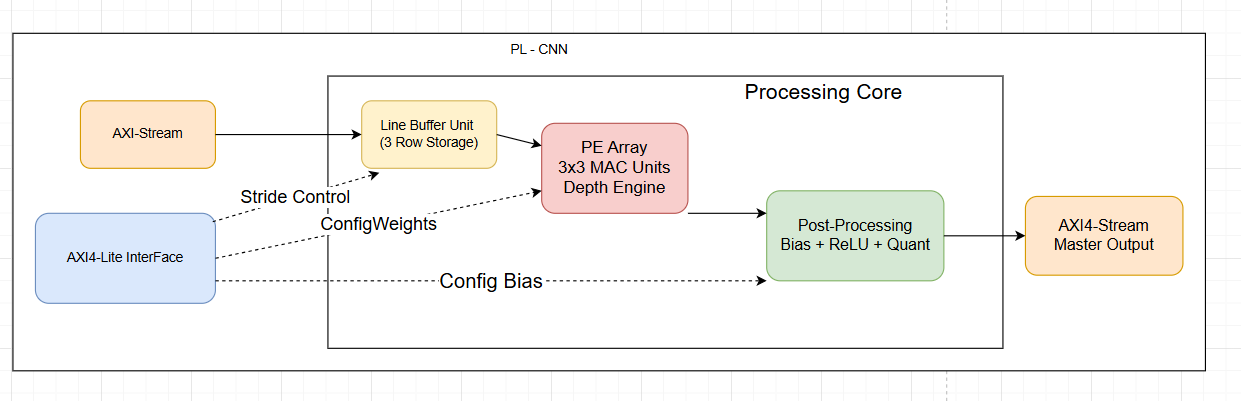
\includegraphics[width=1\textwidth]{images/design/cnn_acce.png}
\caption{Sơ đồ khối chức năng chi tiết của bộ tăng tốc CNN (Accelerator Core Architecture).}
\label{fig:accel_arch}
\end{figure}

\begin{itemize}
    \item \textbf{AXI4-Stream Slave:} Nhận dòng pixel ảnh đầu vào từ uDMA hoặc trực tiếp từ bộ nhớ đệm.
    \item \textbf{AXI4-Stream Master:} Đẩy dòng kết quả (Feature Maps) sau khi tính toán trở lại bộ nhớ.
\end{itemize}

\subsection{Các thành phần chức năng chi tiết}

\subsubsection{Bộ đệm dòng (Line Buffer Unit)}
Do đặc thù của phép tích chập $3 \times 3$ trong MobileNet, tại một thời điểm cần truy cập đồng thời các điểm ảnh thuộc 3 hàng liên tiếp. 
\begin{itemize}
    \item \textbf{Vấn đề:} Nếu đọc từ RAM từng pixel cho mỗi lần trượt cửa sổ, băng thông bộ nhớ sẽ bị quá tải.
    \item \textbf{Giải pháp:} Thiết kế sử dụng cơ chế \textit{Line Buffer} (Bộ đệm dòng) dựa trên BRAM nội bộ. Khi một pixel mới đi vào, nó đẩy các pixel cũ lên các hàng trên (Shift Register). Điều này cho phép tái sử dụng dữ liệu cục bộ, giảm nhu cầu truy cập RAM xuống 3 lần.
\end{itemize}

\subsubsection{Mảng tính toán (Processing Element Array - PE)}
Đây là trung tâm tính toán của Accelerator, được tối ưu cho phép \textbf{Tích chập tách biệt chiều sâu (Depthwise Convolution)}:
\begin{itemize}
    \item Cấu trúc bao gồm 9 bộ nhân (Multipliers) hoạt động song song, tương ứng với Kernel $3 \times 3$.
    \item Các phép toán được thực hiện trên định dạng số nguyên 8-bit (\texttt{int8}) để tiết kiệm tài nguyên DSP Slice trên FPGA.
    \item Kết quả của 9 phép nhân được cộng dồn (Accumulate) để tạo ra một điểm ảnh đầu ra trong mỗi chu kỳ xung nhịp (Single-cycle throughput).
\end{itemize}

\subsubsection{Khối xử lý phi tuyến và Lượng tử hóa (Post-Processing Unit)}
Sau khi tính tổng chập, dữ liệu cần đi qua các bước hậu xử lý trước khi xuất ra ngoài:
\begin{enumerate}
    \item \textbf{Bias Addition:} Cộng giá trị Bias (được nạp trước vào thanh ghi cấu hình).
    \item \textbf{ReLU Activation:} Áp dụng hàm kích hoạt $f(x) = max(0, x)$. Trên phần cứng, đây đơn giản là bộ so sánh với 0 (Multiplexer).
    \item \textbf{Re-Quantization:} Kết quả cộng dồn có thể lên tới 32-bit. Khối này thực hiện nhân với tỷ lệ (Scale factor) và dịch bit (Bit shift) để đưa dữ liệu trở về dạng 8-bit, sẵn sàng cho lớp mạng tiếp theo.
\end{enumerate}

\subsection{Tối ưu hóa cho MobileNetV1}
Thiết kế này giải quyết hai nút thắt chính của MobileNet trên phần cứng:
\begin{itemize}
    \item \textbf{Hỗ trợ Stride = 2:} Accelerator có logic điều khiển để tự động bỏ qua các pixel khi thực hiện giảm kích thước ảnh (Downsampling), giúp giảm 75\% khối lượng tính toán ở các lớp đầu của mạng.
    \item \textbf{Pipelining:} Toàn bộ quá trình từ nạp dữ liệu $\rightarrow$ Line Buffer $\rightarrow$ PE $\rightarrow$ ReLU $\rightarrow$ Xuất dữ liệu được thiết kế theo dạng đường ống (Pipeline). Khi ống đầy, hệ thống đạt hiệu suất 1 kết quả/1 chu kỳ xung nhịp.
\end{itemize}

%=============================================================
%
%=============================================================
\newpage
\section{Thuật toán AI và Thiết kế Phần mềm}
\label{sec:ai_algorithm}

Hệ thống được thiết kế để triển khai mạng nơ-ron tích chập \textbf{MobileNetV1}, 
một kiến trúc được tối ưu hóa cho các thiết bị di động với đặc trưng là sử dụng các 
lớp tích chập tách biệt theo chiều sâu (Depthwise Separable Convolution).

\subsection{Đặc tả Kiến trúc Mô hình}

\begin{figure}[!h]
\centering
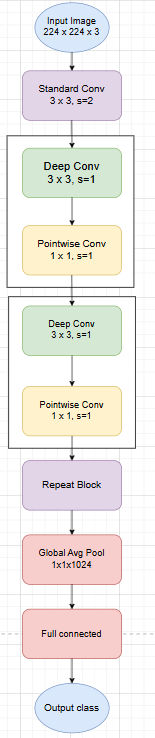
\includegraphics[width=0.2\textwidth]{images/design/conv.png}
\caption{Sơ đồ khối tích chập}
\label{fig:mobilenetv1_arch}
\end{figure}

\newpage

Mô hình được cấu hình với các siêu tham số (Hyperparameters) đầu vào như sau:
\begin{itemize}
    \item \textbf{Kích thước đầu vào (Input Shape):} $224 \times 224 \times 3$ (RGB Image).
    \item \textbf{Độ sâu màu (Bit-depth):} 8-bit Integer (sau khi lượng tử hóa).
    \item \textbf{Tổng số tham số (Parameters):} Xấp xỉ 4.2 triệu tham số.
    \item \textbf{Số lượng phép tính (MACs):} Xấp xỉ 569 triệu phép nhân-cộng.
\end{itemize}


Cấu trúc chi tiết của các lớp mạng và kích thước ma trận Kernel tương ứng được trình bày trong Bảng \ref{tab:mobilenet_layers}. Toàn bộ mạng bao gồm 28 lớp tính toán (nếu tách riêng Depthwise và Pointwise).

\begin{table}[h]
\centering
\caption{Cấu trúc chi tiết các lớp mạng MobileNetV1}
\label{tab:mobilenet_layers}
\resizebox{\textwidth}{!}{%
\begin{tabular}{|l|l|l|l|l|}
\hline
\textbf{Loại Lớp (Layer Type)} & \textbf{Kích thước Input} & \textbf{Kích thước Kernel} & \textbf{Stride} & \textbf{Số kênh Output} \\ \hline
Conv2D (Standard) & $224 \times 224 \times 3$ & $3 \times 3 \times 3 \times 32$ & 2 & 32 \\ \hline
\textbf{Depthwise Conv} & $112 \times 112 \times 32$ & $3 \times 3 \times 32$ (dw) & 1 & 32 \\ \hline
\textbf{Pointwise Conv} & $112 \times 112 \times 32$ & $1 \times 1 \times 32 \times 64$ & 1 & 64 \\ \hline
Depthwise Conv & $112 \times 112 \times 64$ & $3 \times 3 \times 64$ (dw) & 2 & 64 \\ \hline
Pointwise Conv & $56 \times 56 \times 64$ & $1 \times 1 \times 64 \times 128$ & 1 & 128 \\ \hline
Depthwise Conv & $56 \times 56 \times 128$ & $3 \times 3 \times 128$ (dw) & 1 & 128 \\ \hline
Pointwise Conv & $56 \times 56 \times 128$ & $1 \times 1 \times 128 \times 128$ & 1 & 128 \\ \hline
Depthwise Conv & $56 \times 56 \times 128$ & $3 \times 3 \times 128$ (dw) & 2 & 128 \\ \hline
Pointwise Conv & $28 \times 28 \times 128$ & $1 \times 1 \times 128 \times 256$ & 1 & 256 \\ \hline
... (Lặp lại cấu trúc) & ... & ... & ... & ... \\ \hline
Global Avg Pool & $7 \times 7 \times 1024$ & $7 \times 7$ & 1 & 1024 \\ \hline
Fully Connected & $1 \times 1 \times 1024$ & $1 \times 1 \times 1024 \times 1000$ & - & 1000 \\ \hline
\end{tabular}%
}
\end{table}

\subsection{Lượng tử hóa (Quantization)}
Vi xử lý RISC-V và Khối tăng tốc phần cứng trên FPGA được thiết kế để xử lý số nguyên (Integer Arithmetic) nhằm tối đa hóa tốc độ và tiết kiệm bộ nhớ. Do đó, mô hình gốc (Float32) cần trải qua quy trình \textit{Post-training Quantization}:

\begin{itemize}
    \item \textbf{Weights (Trọng số):} Chuyển đổi từ \texttt{float32} (4 bytes) sang \texttt{int8} (1 byte).
    \item \textbf{Activations (Giá trị kích hoạt):} Đầu ra của mỗi lớp cũng được ép về \texttt{int8}.
    \item \textbf{Bias (Hệ số chệch):} Lưu trữ dưới dạng \texttt{int32} để tránh tràn số (overflow) khi cộng dồn, sau đó được dịch bit (bit-shift) để quay về \texttt{int8}.
\end{itemize}

Công thức lượng tử hóa tổng quát được áp dụng:
\begin{equation}
    R = S(Q - Z)
\end{equation}
Trong đó $R$ là giá trị thực (Real value), $Q$ là giá trị lượng tử hóa (Quantized value), $S$ là tỷ lệ (Scale) và $Z$ là điểm không (Zero-point).

\subsection{Tổ chức Dữ liệu trong Bộ nhớ}
Để tối ưu hóa cho việc truy cập Burst qua AXI4 Bus (128-bit width), các ma trận trọng số (Weights) không được lưu trữ theo thứ tự tuyến tính thông thường mà được sắp xếp lại (Memory Packing):
\begin{itemize}
    \item \textbf{Kernel Layout:} Các bộ lọc được sắp xếp theo cấu trúc \texttt{OHWI} 
    (Output-Height-Width-Input) để đảm bảo khi uDMA đọc 16 bytes (128-bit) sẽ thu được 
    đủ dữ liệu cho các bộ nhân hoạt động song song.
    \item \textbf{C-Header Generation:} File mô hình \texttt{.tflite} cuối cùng được
     chuyển đổi (dump) thành các mảng hằng số trong ngôn ngữ C (\texttt{weights.h})
      để biên dịch cùng với Firmware của RISC-V.
\end{itemize}

%=============================================================
\section{Luồng thực thi và Giao thức bắt tay}
\label{sec:system_flow}

Trong kiến trúc SoC dị thể, việc đồng bộ hóa giữa vi xử lý chủ (Host ARM) chạy hệ điều hành và vi xử lý điều khiển (RISC-V) chạy bare-metal là yếu tố then chốt. Hệ thống sử dụng cơ chế bắt tay (Handshaking) dựa trên trạng thái bộ nhớ để đảm bảo tính toàn vẹn dữ liệu.

\paragraph{Định nghĩa Thanh ghi Trạng thái (Mailbox Protocol)}
Vùng nhớ Mailbox tại địa chỉ vật lý \texttt{0xA000\_0000} đóng vai trò là cờ hiệu giao tiếp (Semaphore). Các mã trạng thái được quy ước thống nhất giữa hai vi xử lý như trình bày trong Bảng \ref{tab:mailbox_states}.

\begin{table}[h]
\centering

\begin{tabular}{|c|l|l|}
\hline
\textbf{Mã (Hex)} & \textbf{Trạng thái (State)} & \textbf{Mô tả ý nghĩa} \\ \hline
\texttt{0x00} & \textbf{IDLE} & Hệ thống ở trạng thái nghỉ. PL chờ lệnh từ PS. \\ \hline
\texttt{0x01} & \textbf{DATA\_READY} & PS đã ghi xong dữ liệu ảnh vào DDR và yêu cầu xử lý. \\ \hline
\texttt{0x02} & \textbf{BUSY} & PL đã nhận lệnh và đang thực thi suy luận AI. \\ \hline
\texttt{0x03} & \textbf{DONE} & PL hoàn tất xử lý. Kết quả đã sẵn sàng tại vùng nhớ Output. \\ \hline
\texttt{0xEE} & \textbf{ERROR} & Báo lỗi (ví dụ: Timeout hoặc lỗi phần cứng). \\ \hline
\end{tabular}
\caption{Quy ước mã trạng thái trong giao thức bắt tay PS-PL}
\label{tab:mailbox_states}
\end{table}

\paragraph{Quy trình xử lý một khung hình (Inference Cycle)}
Hoạt động của hệ thống diễn ra theo chu trình khép kín bao gồm 4 giai đoạn chính, 
được minh họa chi tiết trong Sơ đồ tuần tự Hình \ref{fig:sequence_diagram}:

\begin{enumerate}
    \item \textbf{Phần: Thu thập và Tiền xử lý (Host)}
    \begin{itemize}
        \item CPU ARM thu thập hình ảnh từ Camera qua giao diện MIPI CSI-2.
        \item Ảnh được thay đổi kích thước (Resize) về $224 \times 224$ và 
        chuyển đổi không gian màu (nếu cần).
        \item Dữ liệu pixel thô được ghi vào vùng đệm chia sẻ (Shared DDR) 
        tại địa chỉ \texttt{0x4000\_0000}.
        \item ARM ghi giá trị \texttt{0x01} vào Mailbox để kích hoạt PL.
    \end{itemize}

    \item \textbf{Phần: Tiếp nhận và Cấu hình (Controller)}
    \begin{itemize}
        \item Vi xử lý RISC-V (đang trong vòng lặp kiểm tra trạng thái) phát 
        hiện mã \texttt{0x01}.
        \item RISC-V lập tức ghi mã \texttt{0x02} (BUSY) vào Mailbox để khóa 
        tài nguyên.
        \item RISC-V cấu hình bộ điều khiển uDMA: thiết lập địa chỉ nguồn (DDR) 
        và địa chỉ đích (Accelerator Stream Interface).
    \end{itemize}

    \item \textbf{Phần 3: Tăng tốc phần cứng (Accelerator)}
    \begin{itemize}
        \item uDMA bắt đầu truyền dòng dữ liệu (Stream) vào bộ đệm dòng (Line Buffer) 
        của Accelerator.
        \item Mảng tính toán (PE Array) thực hiện tích chập song song.
        \item Kết quả đầu ra được ghi ngược lại vào vùng nhớ Output trong DDR.
        \item Khi hoàn tất toàn bộ các lớp mạng, RISC-V ghi mã \texttt{0x03} (DONE) 
        vào Mailbox.
    \end{itemize}

    \item \textbf{Phần 4: Hậu xử lý và Hiển thị (Host)}
    \begin{itemize}
        \item ARM phát hiện mã \texttt{0x03}, đọc kết quả phân lớp (Label Index) từ DDR.
        \item ARM thực hiện Reset Mailbox về \texttt{0x00} (IDLE) để sẵn sàng cho khung hình tiếp theo.
        \item Kết quả được hiển thị lên màn hình hoặc gửi qua mạng.
    \end{itemize}
\end{enumerate}

\begin{figure}[!h]
    \centering
    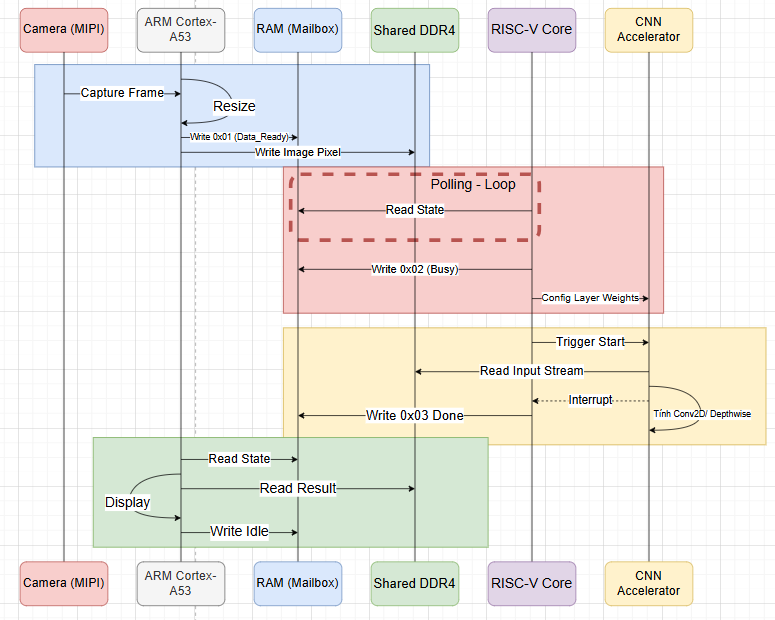
\includegraphics[width=1\textwidth]{images/design/flow.png}
    \caption{Sơ đồ quy trình}
    \label{fig:sequence_diagram}
\end{figure}
\chapter{Hiện thực}

\section{Thiết lập môi trường phát triển}
\label{sec:dev_setup}

\subsection{Nền tảng Phần cứng}
Hệ thống được triển khai và kiểm thử trên bộ kít phát triển \textbf{Xilinx Kria KV260 Vision AI Starter Kit}. Đây là nền tảng chuyên dụng cho các ứng dụng thị giác máy tính tại biên (Edge AI).
\begin{itemize}
    \item \textbf{System-on-Module (SOM):} Kria K26 SOM chứa chip Zynq UltraScale+ MPSoC (XCK26).
    \item \textbf{Tài nguyên:} 4GB RAM DDR4 (dùng chung cho PS và PL), 4 nhân ARM Cortex-A53 và khối logic FPGA với 256K Logic Cells.
    \item \textbf{Ngoại vi:} Camera MIPI CSI-2 (Raspberry Pi Camera V2), cổng Ethernet 1G, và cổng DisplayPort.
\end{itemize}


\subsection{Bộ công cụ thiết kế của Xilinx (Xilinx Design Tools)}
Quy trình thiết kế phần cứng và hệ điều hành được thực hiện trên phiên bản 
sử dụng \textbf{2023.2} để đảm bảo tính tương thích:

\begin{enumerate}
    \item \textbf{Vivado Design Suite:} Sử dụng để thiết kế kiến trúc phần cứng 
    (Block Design), tổng hợp mạch (Synthesis) và tạo bitstream cấu hình cho FPGA.
    \item \textbf{Vitis Unified Software Platform:} Dùng để phát triển Firmware 
    bare-metal và các ứng dụng tăng tốc phần cứng.
    \item \textbf{PetaLinux Tools:} Bộ công cụ xây dựng hệ điều hành 
    Linux nhúng tùy biến.
\end{enumerate}

\subsection{Môi trường biên dịch RISC-V (RISC-V Toolchain)}
Khác với các vi xử lý RISC-V tiêu chuẩn, nhân PULP sử dụng tập 
lệnh mở rộng để tăng tốc DSP và vòng lặp. Do đó, hệ thống yêu cầu bộ biên dịch 
chuyên biệt \texttt{pulp-riscv-gnu-toolchain}.

\begin{itemize}
    \item \textbf{Compiler:} \texttt{riscv32-unknown-elf-gcc}.
    \item \textbf{Cấu hình Build:} Hỗ trợ kiến trúc \texttt{rv32imcxpulpv2} 
    (Tập lệnh cơ bản + Nhân + Nén + Mở rộng PULP).
    \item \textbf{Thư viện:} Newlib (thư viện C chuẩn rút gọn cho hệ thống nhúng).
\end{itemize}

%============================================================
%
%============================================================
\section{Quy trình triển khai hệ thống}
\label{sec:workflow}

Để hiện thực hóa một hệ thống SoC phức tạp kết hợp giữa phần cứng tùy biến (FPGA) 
và phần mềm nhúng (Embedded Software), quá trình triển khai được chia thành 
5 giai đoạn tuần tự theo mô hình thiết kế dựa trên nền tảng (Platform-based Design). 

\subsection{Mô tả các giai đoạn}

Quá trình hiện thực được thực hiện lần lượt theo các bước sau:

\begin{enumerate}
    \item \textbf{Giai đoạn 1: Chuẩn bị Môi trường (Setup \& Toolchain)}
    \begin{itemize}
        \item Cài đặt và cấu hình các công cụ cốt lõi: Vivado (Phần cứng), Vitis (Phần mềm), PetaLinux (Hệ điều hành).
        \item Thiết lập chuỗi công cụ biên dịch chéo (Cross-compiler Toolchain) cho kiến trúc RISC-V PULP.
    \end{itemize}

    \item \textbf{Giai đoạn 2: Tối ưu hóa Mô hình AI (Model Optimization)}
    \begin{itemize}
        \item Huấn luyện và tinh chỉnh (Fine-tune) mạng MobileNetV1 trên máy tính cá nhân (Host PC).
        \item Thực hiện lượng tử hóa (Quantization) từ Float32 sang Int8.
        \item Xuất mô hình dưới dạng mảng dữ liệu C (Weights/Bias Header files) để sẵn sàng nhúng xuống phần cứng.
    \end{itemize}

    \item \textbf{Giai đoạn 3: Thiết kế Phần cứng SoC (Hardware Implementation)}
    \begin{itemize}
        \item Tích hợp IP Core RISC-V và khối tăng tốc CNN Accelerator vào nền tảng Zynq UltraScale+ trên Vivado.
        \item Thiết lập các kết nối AXI Interconnect, xung nhịp và bản đồ địa chỉ.
        \item Tổng hợp mạch (Synthesis), thực thi (Implementation) và tạo Bitstream (.bit).
    \end{itemize}

    \item \textbf{Giai đoạn 4: Phát triển Phần mềm Nhúng (Firmware \& OS)}
    \begin{itemize}
        \item Xây dựng hệ điều hành Linux tùy biến bằng PetaLinux, kích hoạt các driver cần thiết (UIO, CMA).
        \item Viết chương trình Firmware (Bare-metal) cho RISC-V để điều khiển khối Accelerator.
        \item Viết ứng dụng quản lý trên ARM (Python/C++) để giao tiếp và hiển thị kết quả.
    \end{itemize}

    \item \textbf{Giai đoạn 5: Tích hợp và Kiểm thử (Integration \& Verification)}
    \begin{itemize}
        \item Nạp Bitstream và khởi động hệ thống trên board Kria KV260.
        \item Chạy thực nghiệm với Video đầu vào từ Camera.
        \item Đo đạc thông số: Tốc độ (FPS), Độ chính xác (Accuracy) và Tài nguyên sử dụng.
    \end{itemize}
\end{enumerate}
%============================================================
%
%============================================================
\newpage
\section{Huấn luyện và tối ưu hóa Mô hình AI}

\subsection{Chuẩn bị Dữ liệu (Dataset)}
Hệ thống sử dụng bộ dữ liệu "Human Detection Dataset" từ Kaggle: 
\href{https://www.kaggle.com/datasets/jcoral02/inriaperson}{Kaggle - INRIA Person Dataset}
, bao gồm gần 300 ảnh 
ảnh có gán nhãn (Labeled) với hai lớp: \texttt{Human} và \texttt{Background}. 
Dữ liệu được chia theo tỷ lệ 80:20 cho huấn luyện và kiểm thử.

\subsection{Huấn luyện (Training Process)}
Quá trình huấn luyện sử dụng kỹ thuật Transfer Learning trên nền tảng TensorFlow/Keras:
\begin{itemize}
    \item \textbf{Base Model:} MobileNetV1 ($ \alpha=0.25 $) đã được pre-train trên 
    ImageNet. Các lớp tích chập được đóng băng (Freeze).
    \item \textbf{Top Layer:} Thêm lớp Fully Connected mới để phân loại 2 lớp.
    \item \textbf{Loss Function:} Binary Cross-Entropy.
\end{itemize}

% % Chèn đoạn code Python train mô hình (minh họa)
% \begin{lstlisting}[language=Python, caption=Cấu hình Transfer Learning cho MobileNet]
% base_model = tf.keras.applications.MobileNet(
%     input_shape=(224, 224, 3), alpha=0.25, include_top=False, weights='imagenet')
% base_model.trainable = False 

% model = tf.keras.Sequential([
%   base_model,
%   tf.keras.layers.GlobalAveragePooling2D(),
%   tf.keras.layers.Dense(1, activation='sigmoid')
% ])
% \end{lstlisting}

\subsection{Lượng tử hóa và Chuyển đổi (Quantization \& Conversion)}
Để triển khai mô hình trên vi xử lý RISC-V không có bộ xử lý số thực (FPU) mạnh mẽ, mô hình cần được chuyển đổi sang định dạng tính toán số nguyên 8-bit (INT8). Quy trình này sử dụng \texttt{TensorFlow Lite Converter}:

\begin{itemize}
    \item \textbf{Full Integer Quantization:} Chuyển đổi toàn bộ trọng số (Weights) và đầu ra các lớp (Activations) về khoảng giá trị [-128, 127].
    \item \textbf{Representative Dataset:} Sử dụng một tập con gồm 100 ảnh từ tập huấn luyện để bộ chuyển đổi hiệu chỉnh (calibrate) dải động (dynamic range) của các tham số.
\end{itemize}

% \begin{lstlisting}[language=Python, caption=Mã chuyển đổi TFLite và Lượng tử hóa]
% # Hàm generator cung cấp dữ liệu mẫu
% def representative_data_gen():
%     for input_value in tf_dataset.take(100):
%         yield [input_value]

% converter = tf.lite.TFLiteConverter.from_keras_model(model)
% converter.optimizations = [tf.lite.Optimize.DEFAULT]
% converter.representative_dataset = representative_data_gen
% # Ép kiểu tính toán và đầu ra về int8
% converter.target_spec.supported_ops = [tf.lite.OpsSet.TFLITE_BUILTINS_INT8]
% converter.inference_input_type = tf.int8
% converter.inference_output_type = tf.int8

% tflite_model_quant = converter.convert()
% # Lưu ra file .tflite
% with open('mobilenet_quant.tflite', 'wb') as f:
%     f.write(tflite_model_quant)
% \end{lstlisting}

\subsection{Xuất dữ liệu sang C Header (Export to C)}
Bước cuối cùng của Phase 1 là chuyển đổi file nhị phân \texttt{.tflite} 
thành các mảng hằng số ngôn ngữ C để nhúng vào Firmware của RISC-V. 
\begin{itemize}
    \item File \texttt{weights.h}: Chứa mảng trọng số.
    \item File \texttt{bias.h}: Chứa các hệ số chệch.
\end{itemize}

Dưới đây là cấu trúc dữ liệu sau khi chuyển đổi, sẵn sàng để nạp vào bộ nhớ FPGA:

% \begin{lstlisting}[language=C, caption=Trích đoạn file weights.h sau khi xuất]
% // File: weights.h
% // MobileNet Quantized Weights
% #include <stdint.h>

% const uint8_t conv1_weights[] __attribute__((aligned(16))) = {
%     0x04, 0xFE, 0x1A, 0x22, ... // Dữ liệu Hex dạng int8
% };

% const int32_t conv1_bias[] = {
%     120, -45, 300, ... // Bias thường lưu ở int32
% };
% \end{lstlisting}

\newpage
\subsection{Kết quả Huấn luyện ban đầu}
Kết quả thực nghiệm trên tập kiểm thử (Test set) cho thấy mô hình sau khi lượng tử hóa vẫn giữ được độ chính xác chấp nhận được cho bài toán phát hiện người:

\begin{table}[!h]
\centering
\begin{tabular}{|l|c|c|c|}
\hline
\textbf{Phiên bản Mô hình} & \textbf{Độ chính xác (Acc)} & \textbf{Kích thước} & \textbf{Ghi chú} \\ \hline
MobileNet (Float32) & 94.5\% & 16.2 MB & Chạy trên PC \\ \hline
MobileNet (Int8) & 92.8\% & 4.1 MB & Giảm 4x kích thước \\ \hline
\end{tabular}
\caption{So sánh hiệu năng mô hình trước và sau lượng tử hóa.}
\label{tab:model_result}
\end{table}

\chapter{Kết luận và Hướng phát triển}
\label{chap:conclusion}

Đồ án đã bước đầu hoàn thành giai đoạn thiết kế và kiểm chứng mô hình 
cho một hệ thống Edge AI hiệu năng cao trên nền tảng FPGA. 
Chương này tổng kết các kết quả đạt được, nghiên cứ phần hiện thực kỹ thuật 
và đề ra lộ trình chi tiết cho giai đoạn hiện thực phần cứng.

\section{Kết quả đạt được}
Trong giai đoạn này, đồ án đã hoàn thành thiết kế kiến trúc hệ thống và 
chuẩn bị tài nguyên phần mềm, cụ thể:

\begin{enumerate}
    \item \textbf{Đề xuất kiến trúc SoC dị thể tối ưu:} Đã thiết kế chi tiết hệ thống tích hợp giữa Vi xử lý ứng dụng (ARM Cortex-A53 trên Zynq UltraScale+), Vi xử lý điều khiển lõi mềm (RISC-V PULP) và Khối tăng tốc phần cứng (CNN Accelerator). Kiến trúc này giải quyết bài toán cân bằng giữa tính linh hoạt và hiệu năng tính toán.
    
    \item \textbf{Thiết kế chi tiết các phân hệ giao tiếp:}
    \begin{itemize}
        \item Quy hoạch thành công bản đồ bộ nhớ (Memory Map) cho hệ thống chia sẻ tài nguyên.
        \item Thiết kế cơ chế giao tiếp liên nhân (Inter-core Communication) sử dụng Mailbox và giao thức bắt tay (Handshaking) để đồng bộ hóa dữ liệu giữa miền PS (Linux) và PL (Bare-metal).
        \item Xây dựng sơ đồ luồng dữ liệu (Dataflow) tối ưu hóa cho truy cập bộ nhớ dạng Burst qua AXI4.
    \end{itemize}

    \item \textbf{Xây dựng và Tối ưu hóa Mô hình AI:}
    \begin{itemize}
        \item Lựa chọn và huấn luyện thành công mạng MobileNetV1 cho bài toán phát hiện người (Human Detection) với độ chính xác khả quan trên tập kiểm thử.
        \item Hoàn tất quy trình Lượng tử hóa (Quantization) từ Float32 sang Int8, giúp giảm 4 lần kích thước mô hình mà không làm giảm đáng kể độ chính xác.
        \item Chuyển đổi thành công mô hình sang định dạng mảng C (Header files), sẵn sàng cho việc nhúng xuống phần cứng.
    \end{itemize}
\end{enumerate}

\section{Khó khăn và Hạn chế}
Trong quá trình thực hiện, nhóm đã gặp phải và xử lý một số thách thức kỹ thuật:

\begin{itemize}
    \item \textbf{Sự phức tạp của giao tiếp AXI:} Việc đồng bộ hóa giữa miền xung nhịp cao (1.2 GHz của ARM) và miền xung nhịp thấp (100 MHz của FPGA) đòi hỏi thiết kế bộ đệm và cơ chế CDC (Clock Domain Crossing) cẩn trọng để tránh mất mát dữ liệu.
    \item \textbf{Thiên kiến dữ liệu (Data Bias):} Các bộ dữ liệu ban đầu (ảnh chân dung/khuôn mặt) không phù hợp với góc nhìn thực tế của Camera giám sát. Vấn đề này đã được khắc phục bằng việc chuyển sang sử dụng bộ dữ liệu chuẩn hóa (như INRIA Person Dataset/COCO) chứa ảnh toàn thân và bối cảnh đa dạng.
    \item \textbf{Giới hạn bộ nhớ nội (On-chip Memory):} Dung lượng BRAM trên FPGA có hạn, đòi hỏi chiến lược quản lý bộ nhớ đệm dòng (Line Buffer) hiệu quả để tối ưu hóa việc tái sử dụng dữ liệu.
\end{itemize}

\newpage
\section{Kế hoạch thực hiện tiếp theo}
Giai đoạn tiếp theo sẽ tập trung vào việc hiện thực hóa thiết kế trên bo mạch vật lý Kria KV260. Các đầu việc chính bao gồm:

\begin{enumerate}
    \item \textbf{Hiện thực Phần cứng (Hardware Implementation):}
    \begin{itemize}
        \item Tiến hành Tổng hợp (Synthesis) và Thực thi (Implementation) thiết kế trên Vivado.
        \item Đóng gói Bitstream và xuất khẩu phần cứng (Hardware Export - XSA).
    \end{itemize}

    \item \textbf{Phát triển Firmware và Hệ điều hành:}
    \begin{itemize}
        \item Xây dựng bản dựng PetaLinux tùy biến, tích hợp driver UIO để truy cập vùng nhớ vật lý.
        \item Lập trình Firmware C cho nhân RISC-V, tích hợp các mảng trọng số đã xuất ra từ Phase 1.
    \end{itemize}

    \item \textbf{Tích hợp và Đánh giá thực nghiệm:}
    \begin{itemize}
        \item Chạy thử nghiệm hệ thống với Camera MIPI CSI-2 theo thời gian thực.
        \item Đo đạc các thông số kỹ thuật quan trọng: Tốc độ xử lý (FPS), Độ trễ (Latency) và Công suất tiêu thụ (Power Consumption).
        \item So sánh hiệu năng giữa việc chạy thuần trên ARM và chạy có tăng tốc phần cứng để minh chứng tính hiệu quả của đề tài.
    \end{itemize}
\end{enumerate}

\textbf{kế hoạch thực hiện}

\begin{figure}[!h]
    \centering
    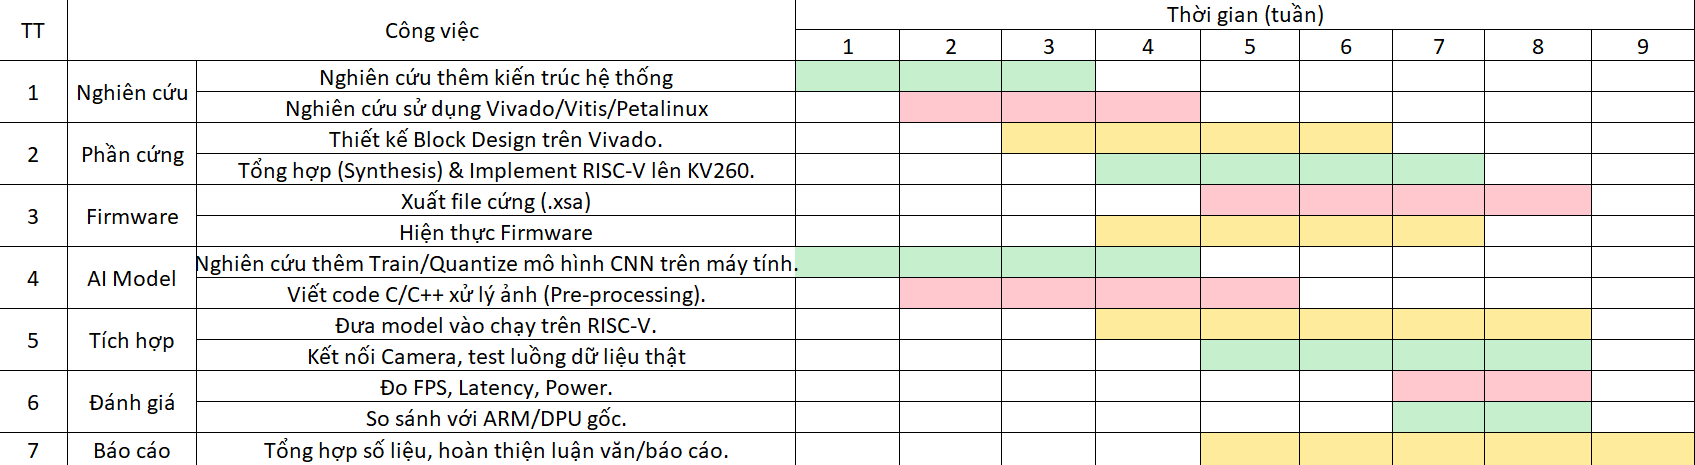
\includegraphics[width=1\textwidth]{images/conclude/gantt.png}
    \caption{Biểu đồ Gantt kế hoạch thực hiện giai đoạn hiện thực}
    \label{fig:gantt_chart}
\end{figure}
% \include{tltk}
\nocite{*}
\printbibliography[heading=bibintoc, title={Tài liệu tham khảo}]
\end{document}